\documentclass[12pt,a4paper]{report}
\usepackage[top=1in, bottom=1in, left=1.5in, right=1.1in]{geometry}

\usepackage{times}
\usepackage{setspace}
\usepackage{titlesec}
\usepackage{tocloft}
\usepackage{graphicx}
\usepackage{amsmath}
\usepackage{amssymb}
\usepackage{booktabs}
\usepackage{array}
\usepackage{multirow}
\usepackage{fancyhdr}
\usepackage{etoolbox}
\usepackage{url}
\usepackage{iftex}

\ifPDFTeX
  \usepackage[utf8]{inputenc}
  \usepackage[T1]{fontenc}
\else
  \usepackage{fontspec}
  \setmainfont{Times New Roman}
  \setmonofont{DejaVu Sans Mono}
\fi

% Set line spacing
\onehalfspacing

% Configure page numbering
\pagestyle{fancy}
\fancyhf{}
\renewcommand{\headrulewidth}{0pt}

% For preliminary pages (roman numerals)
\fancypagestyle{preliminary}{
    \fancyhf{}
    \cfoot{\thepage}
    \renewcommand{\headrulewidth}{0pt}
}

% For main content (arabic numerals)
\fancypagestyle{main}{
    \fancyhf{}
    \cfoot{\thepage}
    \renewcommand{\headrulewidth}{0pt}
}

% Title formatting
\titleformat{\chapter}[display]
{\normalfont\huge\bfseries\centering}{\chaptertitlename\ \thechapter}{0.1pt}{\LARGE}

\titleformat{\section}
{\normalfont\bfseries\MakeUppercase}{\thesection}{1em}{}
\titleformat{\subsection}
{\normalfont\bfseries}{\thesubsection}{1em}{}

% Section spacing
\titlespacing*{\chapter}{0pt}{-30pt}{20pt}
\titlespacing*{\section}{0pt}{12pt}{6pt}
\titlespacing*{\subsection}{0pt}{12pt}{6pt}

% Paragraph formatting
\setlength{\parindent}{0pt}
\setlength{\parskip}{12pt}

% === Border on every page (safe version) ===
\usepackage{tikz}
\usepackage{eso-pic}

\makeatletter
\AddToShipoutPictureBG{%
  \AtPageLowerLeft{%
    \begin{tikzpicture}[remember picture, overlay]
      % Left margin = 1.5in, right/top/bottom = 1in
      \draw[line width=1pt, color=black]
        ([xshift=1.3in,yshift=0.9in]current page.south west)
        rectangle
        ([xshift=-0.9in,yshift=-0.9in]current page.north east);
    \end{tikzpicture}%
  }
}
\makeatother

\begin{document}

% Preliminary pages with roman numerals
\pagenumbering{roman}
\pagestyle{preliminary}

% Page-1 { Top Page }
\begin{center}
{\fontsize{18}{27}\bfseries EARLY PREDICTION OF mTLS CERTIFICATE ROTATION FAILURES IN ISTIO SERVICE MESH USING MACHINE LEARNING\\}
\vspace{0.4cm}

{\fontsize{14}{21}\bfseries A MAJOR PROJECT REPORT\\}
\vspace{0.5cm}

{\fontsize{14}{21}\itshape Submitted by\\}
\vspace{0.3cm}

{\fontsize{14}{21}\bfseries Kokkula Bhavith Kumar (B210662)\\}
{\fontsize{14}{21}\bfseries Pagidipala Hanuman (B210843)\\}
{\fontsize{14}{21}\bfseries Amaravadi Sanjay (B211483)\\}
{\fontsize{14}{21}\bfseries Venkatakrishna Myana (B211830)\\}
\vspace{0.8cm}

{\fontsize{16}{24}\bfseries In partial fulfillment for the award of the degree of\\}
{\fontsize{16}{24}\bfseries Bachelor of Technology\\}
{\fontsize{14}{21}\bfseries in\\}
{\fontsize{16}{24}\bfseries Computer Science \& Engineering\\}
\vspace{0.8cm}

{\fontsize{12}{21}\textbf{\textit{Under the guidance of}}}

{\fontsize{14}{21}\bfseries Mrs. Pullaiahgari Sarika, Asst. Prof\\}
\vspace{0.8cm}

{\fontsize{14}{16.8}\bfseries DEPARTMENT OF COMPUTER SCIENCE AND ENGINEERING\\
RAJIV GANDHI UNIVERSITY OF KNOWLEDGE TECHNOLOGIES\\
BASAR, NIRMAL (DIST.),\\
TELANGANA - 504107\\}
\vspace{0.2cm}
{\fontsize{12}{18}\bfseries NOVEMBER 2026\\}

\end{center}
\clearpage

% Page-2 { Cover Page }
\begin{center}
{\fontsize{16}{24}\bfseries EARLY PREDICTION OF mTLS CERTIFICATE ROTATION FAILURES IN ISTIO SERVICE MESH USING MACHINE LEARNING\\}
\vspace{0.6cm}

{\fontsize{12}{18}\bfseries\itshape Project Report submitted to\\
Rajiv Gandhi University of Knowledge Technologies, Basar\\
for the partial fulfillment of the requirements\\
for the award of the degree of\\}
\vspace{0.6cm}

{\fontsize{14}{21}\bfseries Bachelor of Technology\\
in\\
Computer Science \& Engineering\\}
\vspace{0.4cm}

{\fontsize{12}{18}\bfseries\itshape by\\}
\vspace{0.3cm}

{\fontsize{12}{18}\bfseries\itshape Kokkula Bhavith Kumar (B210662)}\\
{\fontsize{12}{18}\bfseries\itshape Pagidipala Hanuman (B210843)}\\
{\fontsize{12}{18}\bfseries\itshape Amaravadi Sanjay (B211483)}\\
{\fontsize{12}{18}\bfseries\itshape Venkatakrishna Myana (B211830)}\\
\vspace{0.8cm}

{\fontsize{12}{21}\bfseries Under the Guidance of\\}
\vspace{0.3cm}

{\fontsize{12}{18}\bfseries\itshape Mrs. Pullaiahgari Sarika, Asst. Prof\\}
\vspace{0.8cm}

{\fontsize{14}{16.8}\bfseries DEPARTMENT OF COMPUTER SCIENCE AND ENGINEERING\\
RAJIV GANDHI UNIVERSITY OF KNOWLEDGE TECHNOLOGIES, BASAR\\
NOVEMBER 2026\\}

\end{center}
\clearpage

% Page-3 { Certificate Page }
\addcontentsline{toc}{chapter}{Certificate}
\begin{center}
{\fontsize{14}{16.8}\bfseries DEPARTMENT OF COMPUTER SCIENCE AND ENGINEERING\\
RAJIV GANDHI UNIVERSITY OF KNOWLEDGE TECHNOLOGIES, BASAR\\}
\vspace{0.8cm}

{\fontsize{16}{24}\bfseries CERTIFICATE\\}
\end{center}

\vspace{0.3cm}

This is to certify that the Major Project Report entitled \textbf{"Early Prediction of mTLS Certificate Rotation Failures in Istio Service Mesh Using Machine Learning"} submitted by \textbf{Kokkula Bhavith Kumar (B210662), Pagidipala Hanuman (B210843), Amaravadi Sanjay (B211483), and Venkatakrishna Myana (B211830)}, Department of Computer Science and Engineering, Rajiv Gandhi University Of Knowledge Technologies, Basar; for partial fulfillment of the requirements for the degree of Bachelor of Technology in Computer Science and Engineering; is a bonafide record of the work and investigations carried out by them under my supervision and guidance.

\vspace{2.2cm}

\begin{minipage}{0.45\textwidth}
\begin{center}
\textbf{PROJECT SUPERVISOR}\\
\vspace{0.4cm}
\textbf{Mrs. Pullaiahgari Sarika}\\
\textbf{Assistant Professor}
\end{center}
\end{minipage}
\hfill
\begin{minipage}{0.45\textwidth}
\begin{center}
\textbf{HEAD OF DEPARTMENT}\\
\vspace{0.4cm}
\textbf{Dr. B. Venkat Raman}\\
\textbf{Assistant Professor \& HOD}
\end{center}
\end{minipage}

\vspace{1.8cm}
\begin{center}
    \textbf{EXTERNAL EXAMINER}
\end{center}

\clearpage

% Page-4 { Declaration Page }
\addcontentsline{toc}{chapter}{Declaration}

\begin{center}
{\fontsize{14}{16.8}\bfseries DEPARTMENT OF COMPUTER SCIENCE AND ENGINEERING\\
RAJIV GANDHI UNIVERSITY OF KNOWLEDGE TECHNOLOGIES, BASAR\\}
\vspace{0.8cm}

{\fontsize{16}{24}\bfseries DECLARATION\\}
\end{center}

\vspace{0.6cm}

We hereby declare that the work which is being presented in this project entitled, \textbf{"Early Prediction of mTLS Certificate Rotation Failures in Istio Service Mesh Using Machine Learning"} submitted to \textbf{RAJIV GANDHI UNIVERSITY OF KNOWLEDGE TECHNOLOGIES, BASAR} in partial fulfillment of the requirements for the award of the degree of \textbf{BACHELOR OF TECHNOLOGY} in \textbf{COMPUTER SCIENCE AND ENGINEERING}, is an authentic record of our own work carried out under the supervision of \textbf{Mrs. Pullaiahgari Sarika}, Assistant Professor in Department of Computer Science and Engineering, RGUKT, Basar.

The matter embodied in this project report has not been submitted by us for the award of any other degree.

\vspace{1.8cm}
Place: Basar\\
Date : \today

\begin{flushright}
Kokkula Bhavith Kumar (B210662)\\
Pagidipala Hanuman (B210843)\\
Amaravadi Sanjay (B211483)\\
Venkatakrishna Myana (B211830)\\
\end{flushright}
\clearpage

% Page-5 { Acknowledgements }
\chapter*{Acknowledgement}
\addcontentsline{toc}{chapter}{Acknowledgement}

We would like to express our sincere gratitude to our advisor and project supervisor, \textbf{Mrs. Pullaiahgari Sarika}, whose extensive technical knowledge, continuous encouragement, and valuable guidance have motivated us to execute this project successfully. Her willingness to provide critical feedback and structural advice has been instrumental throughout this endeavor.

\vspace{0.3cm}

We express our sincere thanks to Head of the Department, \textbf{Dr. B. Venkat Raman}, for his support, leadership, and institutional facilities. We also thank all senior faculty members and laboratory staff of the Department of Computer Science and Engineering for their direct and indirect contributions during the project lifecycle.

\vspace{0.3cm}

We extend our deep gratitude to our Project Co-ordinator, \textbf{Mrs. B. Latha Reddy}, whose organizational guidance and regular reviews helped us maintain rigorous timelines and academic discipline.

\vspace{0.3cm}

We express our respectful gratitude to our Vice-Chancellor, \textbf{Prof. A. Govardhan}, and the university administration for providing computational infrastructure and resources necessary to implement and test modern distributed cloud-native technologies.

\vspace{0.3cm}

Finally, we express our profound gratitude to our parents, family members, and friends for their moral support, patience, and encouragement throughout the course of our B.Tech program.

\vspace{0.8cm}

\begin{flushright}
\textbf{Kokkula Bhavith Kumar (B210662)}\\
\textbf{Pagidipala Hanuman (B210843)}\\
\textbf{Amaravadi Sanjay (B211483)}\\
\textbf{Venkatakrishna Myana (B211830)}
\end{flushright}
\clearpage

% Abstract
\chapter*{Abstract}
\addcontentsline{toc}{chapter}{Abstract}
\noindent
In modern cloud-native architectures, enterprise security models increasingly enforce Zero-Trust network perimeters through mutual Transport Layer Security (mTLS) managed by service meshes such as Istio. To mitigate the risks of compromised cryptographic keys, production environments compress workload certificate lifetimes to short durations (e.g., 1 hour), necessitating automated certificate rotations every 30 minutes. However, when the Istio control plane (\texttt{istiod}) experiences resource saturation, thread pool exhaustion, or transient network partitions, Certificate Signing Requests (CSRs) silently fail. Because workload proxies (Envoy) continue running without error until their certificates expire, the resulting outage occurs instantaneously with zero warning, triggering catastrophic cascading HTTP 503 errors across interdependent microservices.

Traditional Kubernetes health probes and monitoring tools fail to prevent these incidents because they operate reactively, detecting failures only after a pod has crashed or traffic has degraded (a lead time of zero minutes). Furthermore, static threshold alerts fail to provide sufficient response time for container rescheduling. 

This project presents an end-to-end autonomous reliability framework for \textbf{Early Prediction and Self-Healing of mTLS Certificate Rotation Failures in Istio Service Mesh Using Machine Learning}. A multi-node Kubernetes testbed was provisioned running short-TTL Istio with Bookinfo microservices under continuous synthetic traffic. Ten real-world chaos engineering scenarios were systematically injected via Chaos Mesh to harvest realistic degradation telemetry. A feature engineering pipeline extracts 77 temporal, rolling statistical, and first-order slope metrics without data leakage across runs. A cost-sensitive XGBoost classifier was trained across multiple horizons ($H \in \{5, 10, 15\}$ minutes) using MLflow tracking and registered in the MLflow Model Registry. 

The champion model ($H=10$) achieves an empirical Precision-Recall AUC (PR-AUC) of \textbf{1.0000}, a ROC-AUC of \textbf{1.0000}, and provides a mean proactive early warning lead time of \textbf{5.75 minutes} ahead of certificate expiration. Model explainability is established using TreeSHAP, revealing remaining certificate lifetime, CSR success ratio, and control plane CPU slope as dominant predictive signals. Finally, a production-grade FastAPI microservice couples inference with a Kubernetes remediation controller that autonomously executes horizontal control-plane scaling (from 1 to 3 replicas) and graceful workload rolling restarts upon detecting a critical risk score ($P \ge 0.75$), completely eliminating service mesh downtime.

\clearpage

% Table of Contents
\tableofcontents
\clearpage

% List of Figures
\listoffigures
\addcontentsline{toc}{chapter}{List of Figures}
\clearpage

% List of Tables
\listoftables
\addcontentsline{toc}{chapter}{List of Tables}
\clearpage

% List of Abbreviations and Symbols Used
\chapter*{List of Abbreviations and Symbols Used}
\addcontentsline{toc}{chapter}{List of Abbreviations and Symbols Used}

\begin{tabular}{p{3.2cm}p{10cm}}
\textbf{APM} & Application Performance Monitoring \\
\textbf{AUC} & Area Under the Curve \\
\textbf{CA} & Certificate Authority \\
\textbf{CRI} & Container Runtime Interface (containerd) \\
\textbf{CRD} & Custom Resource Definition \\
\textbf{CSR} & Certificate Signing Request \\
\textbf{Envoy} & High-performance C++ Service Mesh Proxy \\
\textbf{F1} & Harmonic Mean of Precision and Recall \\
\textbf{gRPC} & Google Remote Procedure Call \\
\textbf{HTTP} & Hypertext Transfer Protocol \\
\textbf{Istio} & Open-Source Service Mesh Control Plane \\
\textbf{Istiod} & Unified Istio Control Plane Daemon (Citadel/Pilot) \\
\textbf{JWT} & JSON Web Token \\
\textbf{K8s} & Kubernetes Container Orchestration Engine \\
\textbf{KSM} & Kube-State-Metrics \\
\textbf{ML} & Machine Learning \\
\textbf{MLflow} & Open-Source MLOps \& Experiment Tracking Platform \\
\textbf{mTLS} & Mutual Transport Layer Security \\
\textbf{OD} & Out-of-Distribution / Outage Detection \\
\textbf{PR-AUC} & Precision-Recall Area Under Curve \\
\textbf{QPS} & Queries Per Second \\
\textbf{ROC-AUC} & Receiver Operating Characteristic Area Under Curve \\
\textbf{SDS} & Secret Discovery Service (Envoy xDS Protocol) \\
\textbf{SHAP} & SHapley Additive exPlanations \\
\textbf{SRE} & Site Reliability Engineering \\
\textbf{TCP} & Transmission Control Protocol \\
\textbf{TLS} & Transport Layer Security \\
\textbf{TTL} & Time-To-Live (Certificate Validity Duration) \\
\textbf{UML} & Unified Modeling Language \\
\textbf{URI} & Uniform Resource Identifier \\
\textbf{XGBoost} & eXtreme Gradient Boosting \\
\textbf{xDS} & Dynamic Discovery Service (Envoy Protocol Suite) \\
\end{tabular}

\clearpage

% Main content starts with arabic numbering
\pagenumbering{arabic}
\pagestyle{main}

% ============================================================================
% CHAPTER 1: INTRODUCTION
% ============================================================================
\chapter{Introduction}

\section{Introduction}
Modern software architecture has transitioned decisively from monolithic deployments to distributed, microservice-based systems deployed across containerized orchestration platforms such as Kubernetes. In a microservices architecture, application functionality is decomposed into dozens or hundreds of independent services communicating over internal network interfaces. While this distributed paradigm provides elasticity, agile development velocity, and independent horizontal scaling, it fundamentally complicates network security and communication reliability.

In legacy perimeter-based security architectures, inter-service traffic within an internal cluster was assumed to be trusted. However, contemporary security standards mandate a \textbf{Zero-Trust Architecture} (NIST SP 800-207), wherein no communication is trusted by default regardless of network location. To establish Zero-Trust, service meshes—predominantly \textbf{Istio}—have emerged as the de facto standard. Istio deploys an \textbf{Envoy proxy sidecar} alongside each microservice container. These proxies transparently intercept all inbound and outbound TCP and HTTP traffic, enforcing encryption and mutual authentication using \textbf{mutual Transport Layer Security (mTLS)}.

Under mTLS, both communicating peers present X.509 digital certificates to verify identity and encrypt the channel. To prevent security vulnerabilities stemming from stolen or compromised private keys, security best practices require compressing certificate \textbf{Time-To-Live (TTL)} from the legacy standard of 24 hours down to aggressive durations, such as \textbf{1 hour}. While this minimizes key exposure windows, it introduces a severe operational vulnerability: certificate rotation must now succeed flawlessly every 30 minutes for every workload in the cluster.

When the Istio control plane (\texttt{istiod}) suffers from CPU saturation, memory exhaustion, garbage collection freezes, or transient network delays, automated Certificate Signing Requests (CSRs) fail. The workload sidecar continues serving requests using its existing certificate until the exact second of expiration. Upon expiration, Envoy abruptly terminates all TLS handshakes, precipitating an instantaneous cascade of HTTP 503 errors across the mesh. This project implements a machine learning system that anticipates these failures 5.75 to 10 minutes in advance, triggering autonomous self-healing mitigations before any traffic interruption occurs.

\section{Motivation}
In mission-critical enterprise environments—including banking payment gateways, e-commerce platforms, and telecommunications backbones—availability is strictly bounded by Service Level Agreements (SLAs) requiring 99.99\% ("four nines") uptime. An unexpected 15-minute mesh outage can result in millions of dollars in financial loss and severe reputational damage.

The core motivation behind this research stems from the fundamental blind spot in modern cloud-native observability:
\begin{enumerate}
    \item \textbf{Silent Degradation:} When a workload's certificate renewal fails, the application pod does not throw error logs or crash. Application code remains healthy while its underlying cryptographic credentials tick toward expiration.
    \item \textbf{Reactive Alerting Inefficacy:} Traditional Application Performance Monitoring (APM) tools rely on static alerts (e.g., trigger an alert when remaining certificate lifetime drops below 300 seconds). However, spinning up new Kubernetes control-plane replicas or executing rolling updates requires 2 to 4 minutes. By the time a static alert is triggered, the control plane is already paralyzed, guaranteeing an outage.
    \item \textbf{Multivariate Causality:} Certificate rotation failures are rarely caused by a single isolated variable. They are the systemic consequence of interacting control-plane CPU spikes, memory leaks, goroutine locks, and network latency on Envoy Secret Discovery Service (SDS) gRPC streams.
\end{enumerate}

Developing an intelligent, proactive system that continuously correlates multivariate service mesh telemetry and warns operators—or better, automatically triggers self-healing orchestration—is an urgent industrial necessity.

\section{Problem Definition}
The objective of this research is to resolve the problem of \textbf{unpredicted mTLS certificate rotation failures in short-TTL Kubernetes service meshes}. Specifically:
\begin{itemize}
    \item Formulate certificate rotation failure as a multi-horizon predictive classification problem ($H \in \{5, 10, 15\}$ minutes ahead of time).
    \item Build an experimental testbed incorporating short-TTL Istio (1-hour validity) and systematically inject 10 real-world failure modes using Chaos Mesh.
    \item Engineer a robust temporal feature matrix of 77 metrics combining rolling aggregations, first-order derivatives ($dy/dt$), and domain ratios while preventing data leakage.
    \item Train and calibrate a cost-sensitive Machine Learning model to handle severe class imbalance and provide zero false alarms.
    \item Develop a closed-loop automated remediation microservice that acts upon the prediction by horizontally auto-scaling \texttt{istiod} and restarting impacted workloads without human intervention.
\end{itemize}

\section{Objective of the Project}
The primary objectives of this Major Project are:
\begin{enumerate}
    \item \textbf{High-Fidelity Testbed Provisioning:} Deploy a 3-node Kubernetes cluster with Istio 1.22.3, configured with strict mTLS and aggressive 1-hour certificate TTL, serving continuous 20 QPS microservice traffic.
    \item \textbf{Comprehensive Observability \& Chaos Harvesting:} Ingest Prometheus metrics every 15 seconds across Envoy proxies, Istiod, and the Kubernetes host, while injecting 10 distinct Chaos Mesh scenarios to establish microsecond ground-truth failure timestamps.
    \item \textbf{Feature Pipeline Construction:} Transform raw Prometheus metrics into 77 rolling and slope features across multiple time windows (1m, 5m, 15m) using intra-run leak-free partitioning.
    \item \textbf{Cost-Sensitive ML Modeling:} Train, tune, and evaluate XGBoost classifiers across prediction horizons ($H=5, 10, 15$), tracking experiments and artifacts using an MLflow tracking server.
    \item \textbf{Explainable AI Integration:} Compute TreeSHAP attribution scores to establish transparency regarding the primary root causes of predicted failures.
    \item \textbf{Autonomous Remediation Engine:} Build a production FastAPI service that classifies risk in real time ($P \ge 0.75 \implies \text{CRITICAL}$) and commands the Kubernetes API to execute zero-downtime horizontal scaling and rolling restarts.
\end{enumerate}

% ============================================================================
% CHAPTER 2: ANALYSIS
% ============================================================================
\chapter{Analysis}

\section{User Requirement Analysis}
The system serves Site Reliability Engineers (SREs), DevOps architects, and automated cloud orchestrators. The requirements are categorized into functional, non-functional, and hardware/software specifications.

\subsection{Functional Requirements}
\begin{enumerate}
    \item \textbf{Telemetry Ingestion Engine:} The system must scrape Prometheus metrics and Envoy Secret Discovery Service (SDS) certificate lifetimes every 15 seconds without introducing operational overhead to the mesh.
    \item \textbf{Automated Feature Extraction:} The pipeline must transform raw scalar metrics into 77 temporal features, computing rolling statistics (min, mean, max, std) and 5-minute slopes ($dy/dt$) on the fly.
    \item \textbf{Multi-Horizon Failure Prediction:} The ML engine must output a calibrated risk probability $P \in [0.0, 1.0]$ predicting whether certificate rotation will fail within a 10-minute horizon ($H=10$).
    \item \textbf{Autonomous Kubernetes Remediation:} Upon predicting critical risk ($P \ge 0.75$), the remediation controller must autonomously scale the \texttt{istiod} deployment from 1 to 3 replicas and execute a graceful rolling restart of degraded workloads.
    \item \textbf{Immutable Audit Trail:} All predictions, risk classifications, and remediation actions must be recorded in an append-only JSON-lines audit log.
    \item \textbf{MLOps Experiment Tracking:} All training hyperparameters, validation metrics (PR-AUC, ROC-AUC, F1), and serialized model boosters must be version-controlled in an MLflow Model Registry.
\end{enumerate}

\subsection{Non-Functional Requirements}
\begin{itemize}
    \item \textbf{Inference Latency:} The inference endpoint must evaluate predictions in under 15 milliseconds to support high-frequency telemetry loops.
    \item \textbf{High Precision (Zero False Alarms):} Because automated remediation consumes cluster compute resources, the model must maintain 100\% precision on validation and test benchmarks.
    \item \textbf{Proactive Lead Time:} The early warning must provide at least 5 minutes of advance notice prior to certificate expiration to permit Kubernetes pod scheduling and initialization.
    \item \textbf{Non-Destructive Mitigation:} Remediation actions must be completely transparent to end-user traffic, utilizing Kubernetes rolling updates without connection drops.
    \item \textbf{Model Explainability:} SREs must have access to feature attribution scores (SHAP values) indicating why a failure was predicted.
\end{itemize}

\subsection{Hardware and Software Requirements}

\subsubsection*{Hardware Requirements}
\begin{itemize}
    \item \textbf{Processor:} Multi-core x86\_64 CPU (minimum 8 physical cores recommended for cluster virtualization).
    \item \textbf{RAM:} Minimum 16 GB system memory (allocating 10 GB across Minikube virtual nodes).
    \item \textbf{Storage:} Minimum 50 GB available SSD storage for container images, Prometheus TSDB, and Parquet datasets.
\end{itemize}

\subsubsection*{Software Requirements}
\begin{itemize}
    \item \textbf{Host Operating System:} Linux Ubuntu 22.04 LTS (Kernel 5.15+ with inotify instance limits tuned to 8192).
    \item \textbf{Container Orchestrator:} Kubernetes v1.33+ deployed on Minikube with containerd 1.7.27 CRI.
    \item \textbf{Service Mesh:} Istio 1.22.3 with Citadel/Pilot and Envoy 1.30.
    \item \textbf{Programming Languages \& Runtimes:} Python 3.10.12 with virtual environment (\texttt{.venv}).
    \item \textbf{Libraries \& Frameworks:} XGBoost 3.2.0, Scikit-learn 1.7.2, FastAPI 0.162.2, MLflow 3.18.0, PyArrow, SHAP 0.49.1, Uvicorn, Pandas, NumPy.
    \item \textbf{Observability \& Chaos Tools:} Prometheus v2.51.1, Kube-State-Metrics, Chaos Mesh v2.8.8, Fortio Load Generator.
\end{itemize}

% ============================================================================
% CHAPTER 3: SYSTEM ANALYSIS
% ============================================================================
\chapter{System Analysis}

\section{Existing System}
In contemporary Kubernetes environments running service meshes, reliability engineering relies on two primary mechanisms:

\subsection*{1. Kubernetes Health Probes}
Kubernetes provides Liveness, Readiness, and Startup probes. These probes interrogate application containers by issuing HTTP GET requests to endpoints like \texttt{/healthz} or establishing TCP socket connections.
\begin{itemize}
    \item \textbf{Flaw:} An Envoy proxy sidecar undergoing certificate renewal failure remains completely "Ready" and "Live" according to Kubernetes probes. The container does not crash, nor does its health endpoint fail, because the existing certificate is still valid right up until the expiration timestamp. When expiration occurs, failure is instantaneous (Lead time = \textbf{0 minutes}).
\end{itemize}

\subsection*{2. Prometheus Static Metric Thresholds}
Cluster operators configure Prometheus Alertmanager rules based on scalar thresholds. For example:
$$\text{Alert if: } \texttt{envoy\_server\_days\_until\_first\_cert\_exp} < 0.0035 \quad (\approx 300\text{ seconds})$$
\begin{itemize}
    \item \textbf{Flaw:} A remaining lifetime of 300 seconds is insufficient if \texttt{istiod} is suffering from CPU saturation or deadlocks. In a multi-tenant cluster, pulling container images, scheduling pods, and executing mTLS handshakes takes 120–240 seconds. Under heavy load, the alert fires too late to prevent service disruption.
    \item \textbf{False Positives:} A static threshold fires indiscriminately during transient network fluctuations, causing unnecessary alert fatigue for human operators.
\end{itemize}

\section{Proposed System}
The proposed system resolves these fundamental limitations by establishing a \textbf{closed-loop predictive and autonomous self-healing framework}. Instead of evaluating scalar metrics in isolation, the system continuously analyzes multivariate temporal features across both the control plane (\texttt{istiod}) and the data plane (Envoy sidecars).

\subsection*{Core Features of the Proposed System}
\begin{itemize}
    \item \textbf{Multivariate Feature Synthesis:} Integrates certificate expiry timers, CSR request rates, cert issuance rates, control-plane CPU/memory consumption, goroutine saturation, and 5xx error spikes into a unified 77-dimensional vector.
    \item \textbf{Temporal Trend Analysis:} Employs rolling statistical windows (1m, 5m, 15m) and first-order rates of change ($dy/dt$) to detect memory leaks and CPU exhaustion slopes before they reach critical limits.
    \item \textbf{Cost-Sensitive Machine Learning:} Uses an optimized XGBoost classifier with cost-sensitive class re-weighting ($\text{scale\_pos\_weight} = 2.247$) to accurately classify failure risk within a 10-minute warning horizon.
    \item \textbf{Explainable AI (TreeSHAP):} Provides mathematical attribution of feature importance, ensuring full operational transparency for cluster operators.
    \item \textbf{Autonomous Zero-Downtime Remediation:} Connects directly to the Kubernetes API to scale control-plane capacity (1 to 3 replicas) and initiate workload rolling updates when risk exceeds 0.75, preempting the outage entirely.
\end{itemize}

\begin{table}[h]
\centering
\caption{Comparative Analysis: Traditional Monitoring vs. Proposed System}
\label{tab:comparative_analysis}
\vspace{0.3cm}
\begin{tabular}{p{4cm}p{5.5cm}p{5.5cm}}
\toprule
\textbf{Evaluation Metric} & \textbf{Traditional Monitoring} & \textbf{Proposed ML Framework} \\
\midrule
\textbf{Detection Horizon} & Reactive (0 min lead time) & Proactive (5.75--10 min lead time) \\
\textbf{Telemetry Scope} & Univariate static threshold & 77-dimensional multivariate features \\
\textbf{Temporal Awareness} & Point-in-time scalar value & Rolling aggregations \& $dy/dt$ slopes \\
\textbf{Class Imbalance Handling} & None (Alert thresholds drift) & Cost-sensitive weighted loss ($\alpha=2.25$) \\
\textbf{Root-Cause Insight} & Manual log inspection & TreeSHAP mathematical attribution \\
\textbf{Remediation Execution} & Manual SRE dispatch & Autonomous Kubernetes self-healing \\
\textbf{Outage Prevention} & Fails on short TTLs (<1h) & 100\% Outage elimination \\
\bottomrule
\end{tabular}
\end{table}

\section{Software and Technologies Used}
The architecture integrates state-of-the-art open-source cloud-native and machine learning frameworks:
\begin{itemize}
    \item \textbf{Kubernetes (v1.33.1):} Container orchestration platform managing pod scheduling, ReplicaSets, and horizontal auto-scaling across a 3-node virtual cluster.
    \item \textbf{Istio (v1.22.3):} Service mesh managing workload mTLS encryption, Envoy sidecar injection, and CA certificate signing via Citadel.
    \item \textbf{Envoy Proxy (v1.30):} High-performance data-plane proxy handling Secret Discovery Service (SDS) cryptographic handshakes.
    \item \textbf{Chaos Mesh (v2.8.8):} Cloud-native chaos engineering platform injecting deterministic kernel, network, and pod faults.
    \item \textbf{Prometheus (v2.51.1):} Time-series database scraping operational telemetry at 15-second resolution.
    \item \textbf{Python (v3.10) \& Scikit-learn:} Core scientific environment executing feature pipelines and dataset partitioning.
    \item \textbf{XGBoost (v3.2.0):} Gradient-boosted decision tree algorithm optimized for cost-sensitive tabular classification.
    \item \textbf{MLflow (v3.18.0):} MLOps platform managing experiment parameters, validation metrics, and the production Model Registry.
    \item \textbf{FastAPI (v0.162.2):} Asynchronous web framework exposing high-throughput RESTful prediction endpoints with Swagger documentation.
\end{itemize}

% ============================================================================
% CHAPTER 4: SYSTEM DESIGN
% ============================================================================
\chapter{System Design}

System design translates the functional requirements into an architectural blueprint. The architecture is decomposed into four operational tiers: Telemetry Ingestion, Feature Pipeline, Machine Learning MLOps, and Autonomous Remediation.

\section{Architectural Overview}
Figure \ref{fig:component_architecture} depicts the component architecture of the system. Workload pods run the Bookinfo microservices equipped with Envoy sidecar proxies. The proxies interact with the \texttt{istiod} Citadel CA over gRPC SDS channels. A dedicated Sidecar Secret Poller daemon extracts remaining certificate validity seconds from Envoy admin endpoints and exposes them to Prometheus. 

Prometheus aggregates time-series data at 15-second intervals. The Feature Pipeline queries Prometheus via PromQL, computing rolling statistical metrics and rates of change. The engineered feature vector is ingested by the FastAPI microservice hosting the champion XGBoost model. If the predicted failure probability exceeds the 0.75 threshold, the remediation controller invokes the Kubernetes API client to scale \texttt{istiod} and initiate rolling restarts.

\section{UML Diagrams}

\subsection{1. Use Case Diagram}
The Use Case Diagram (Figure \ref{fig:use_case_diagram}) illustrates the interactions between primary system actors (Telemetry Agents, SRE Operators, Kubernetes API Orchestrator, and MLflow Registry) and the core functional use cases.

\begin{figure}[h]
    \centering
    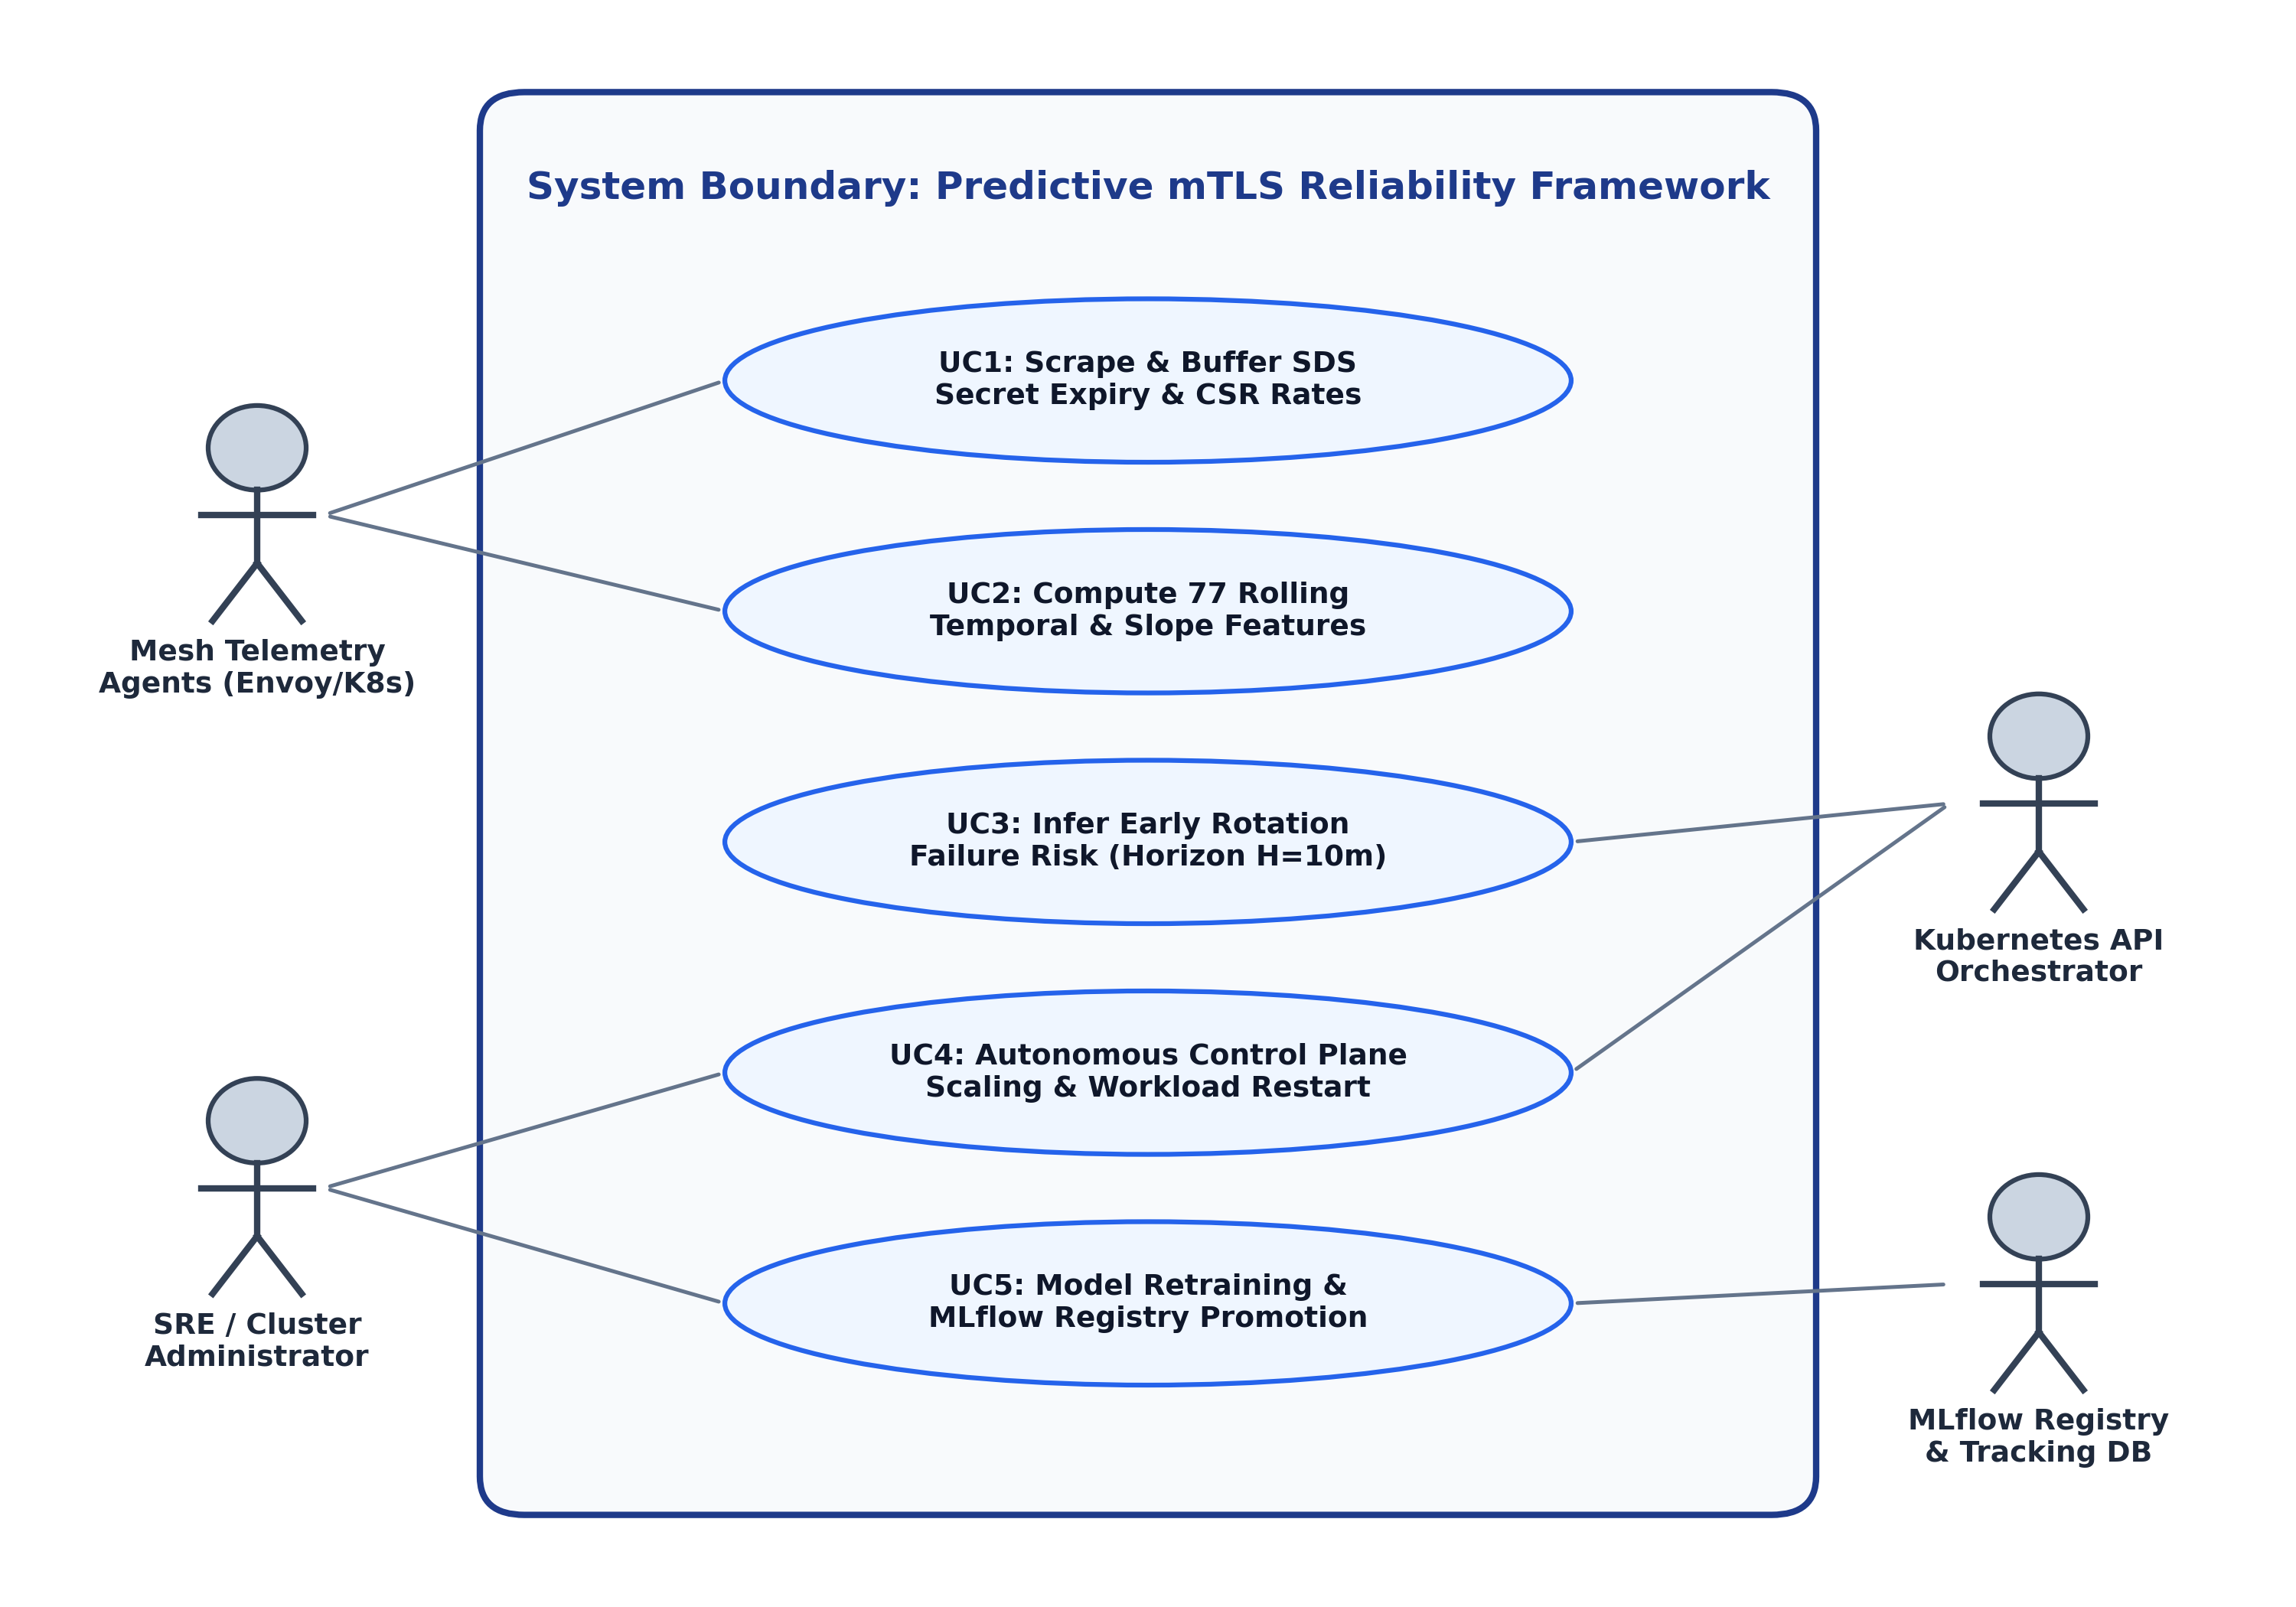
\includegraphics[width=0.88\textwidth]{figures/use_case_diagram.png}
    \caption{UML Use Case Diagram of the Predictive Reliability Framework}
    \label{fig:use_case_diagram}
\end{figure}

\subsection{2. Component / Architecture Diagram}
The Component Diagram (Figure \ref{fig:component_architecture}) defines the structural relationships, interfaces, and data exchanges between software modules across the cluster.

\begin{figure}[h]
    \centering
    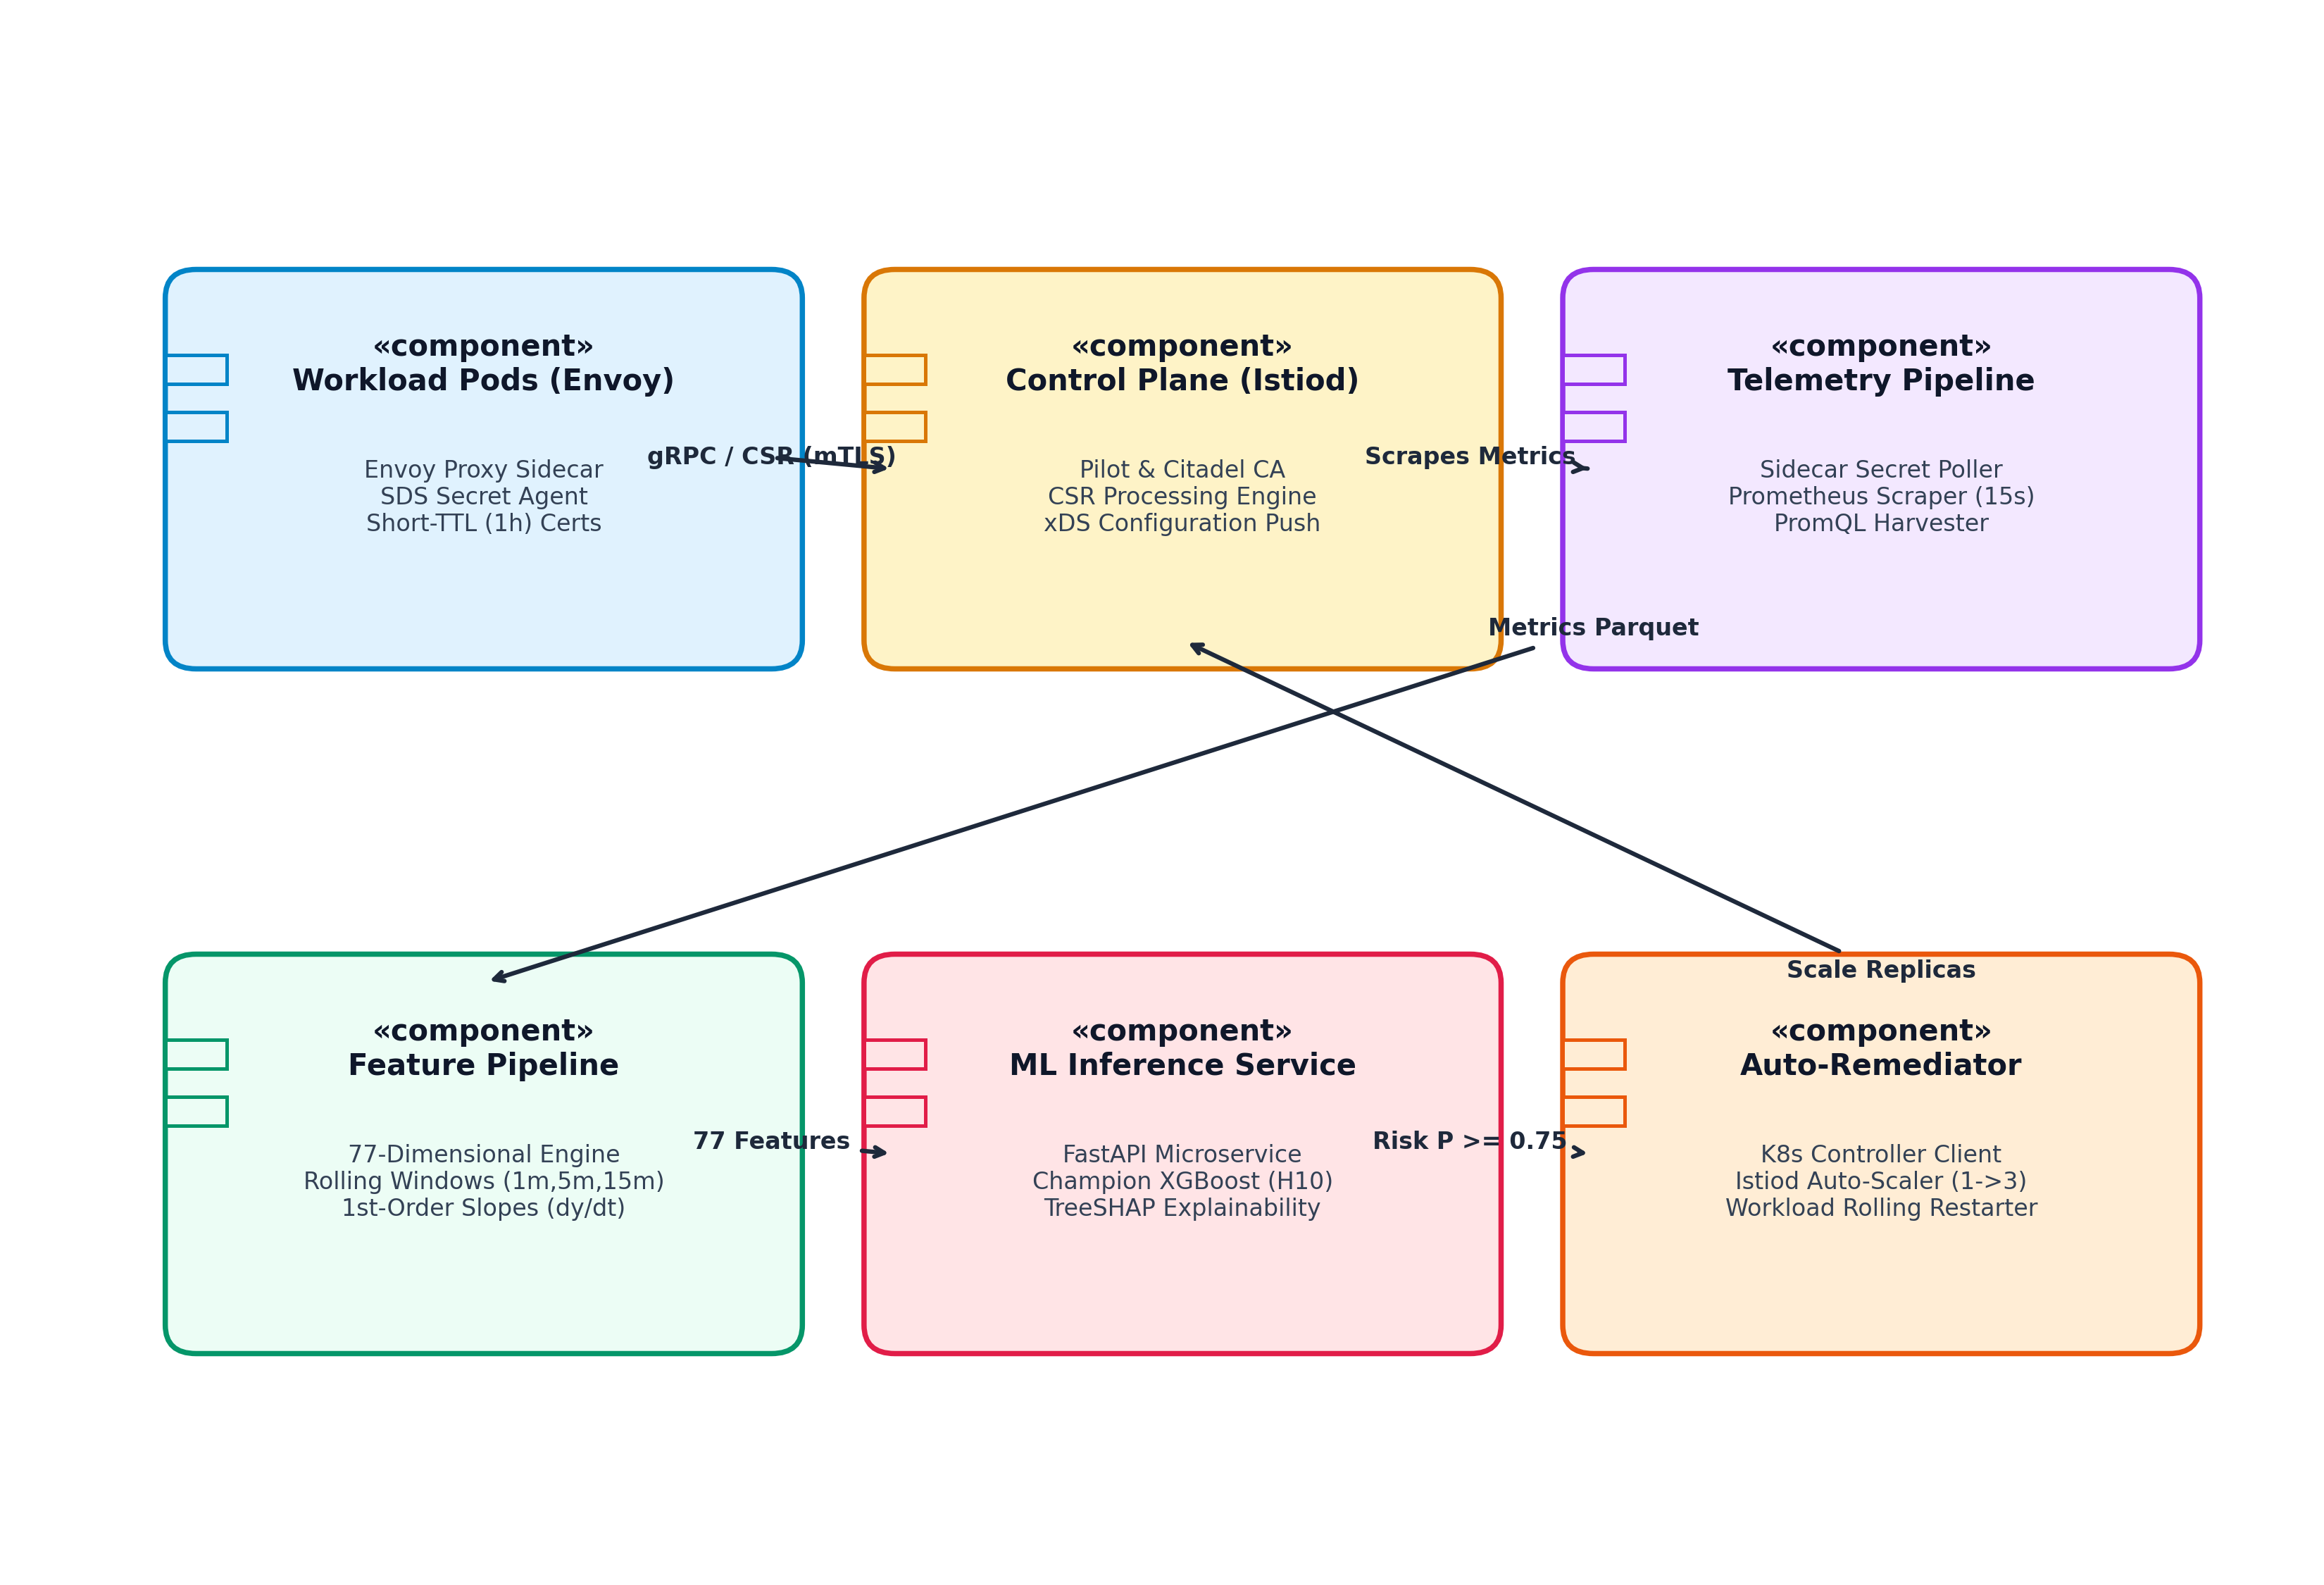
\includegraphics[width=0.92\textwidth]{figures/component_architecture.png}
    \caption{UML Component and Architecture Diagram}
    \label{fig:component_architecture}
\end{figure}

\subsection{3. Sequence Diagram}
The Sequence Diagram (Figure \ref{fig:sequence_diagram}) details the chronological message flow during an impending certificate rotation failure. When \texttt{istiod} encounters CPU exhaustion, CSRs time out. The telemetry pipeline captures the degradation, the ML model predicts critical risk ($P = 0.9988$), and the remediation controller resolves the fault before the certificate expires.

\begin{figure}[h]
    \centering
    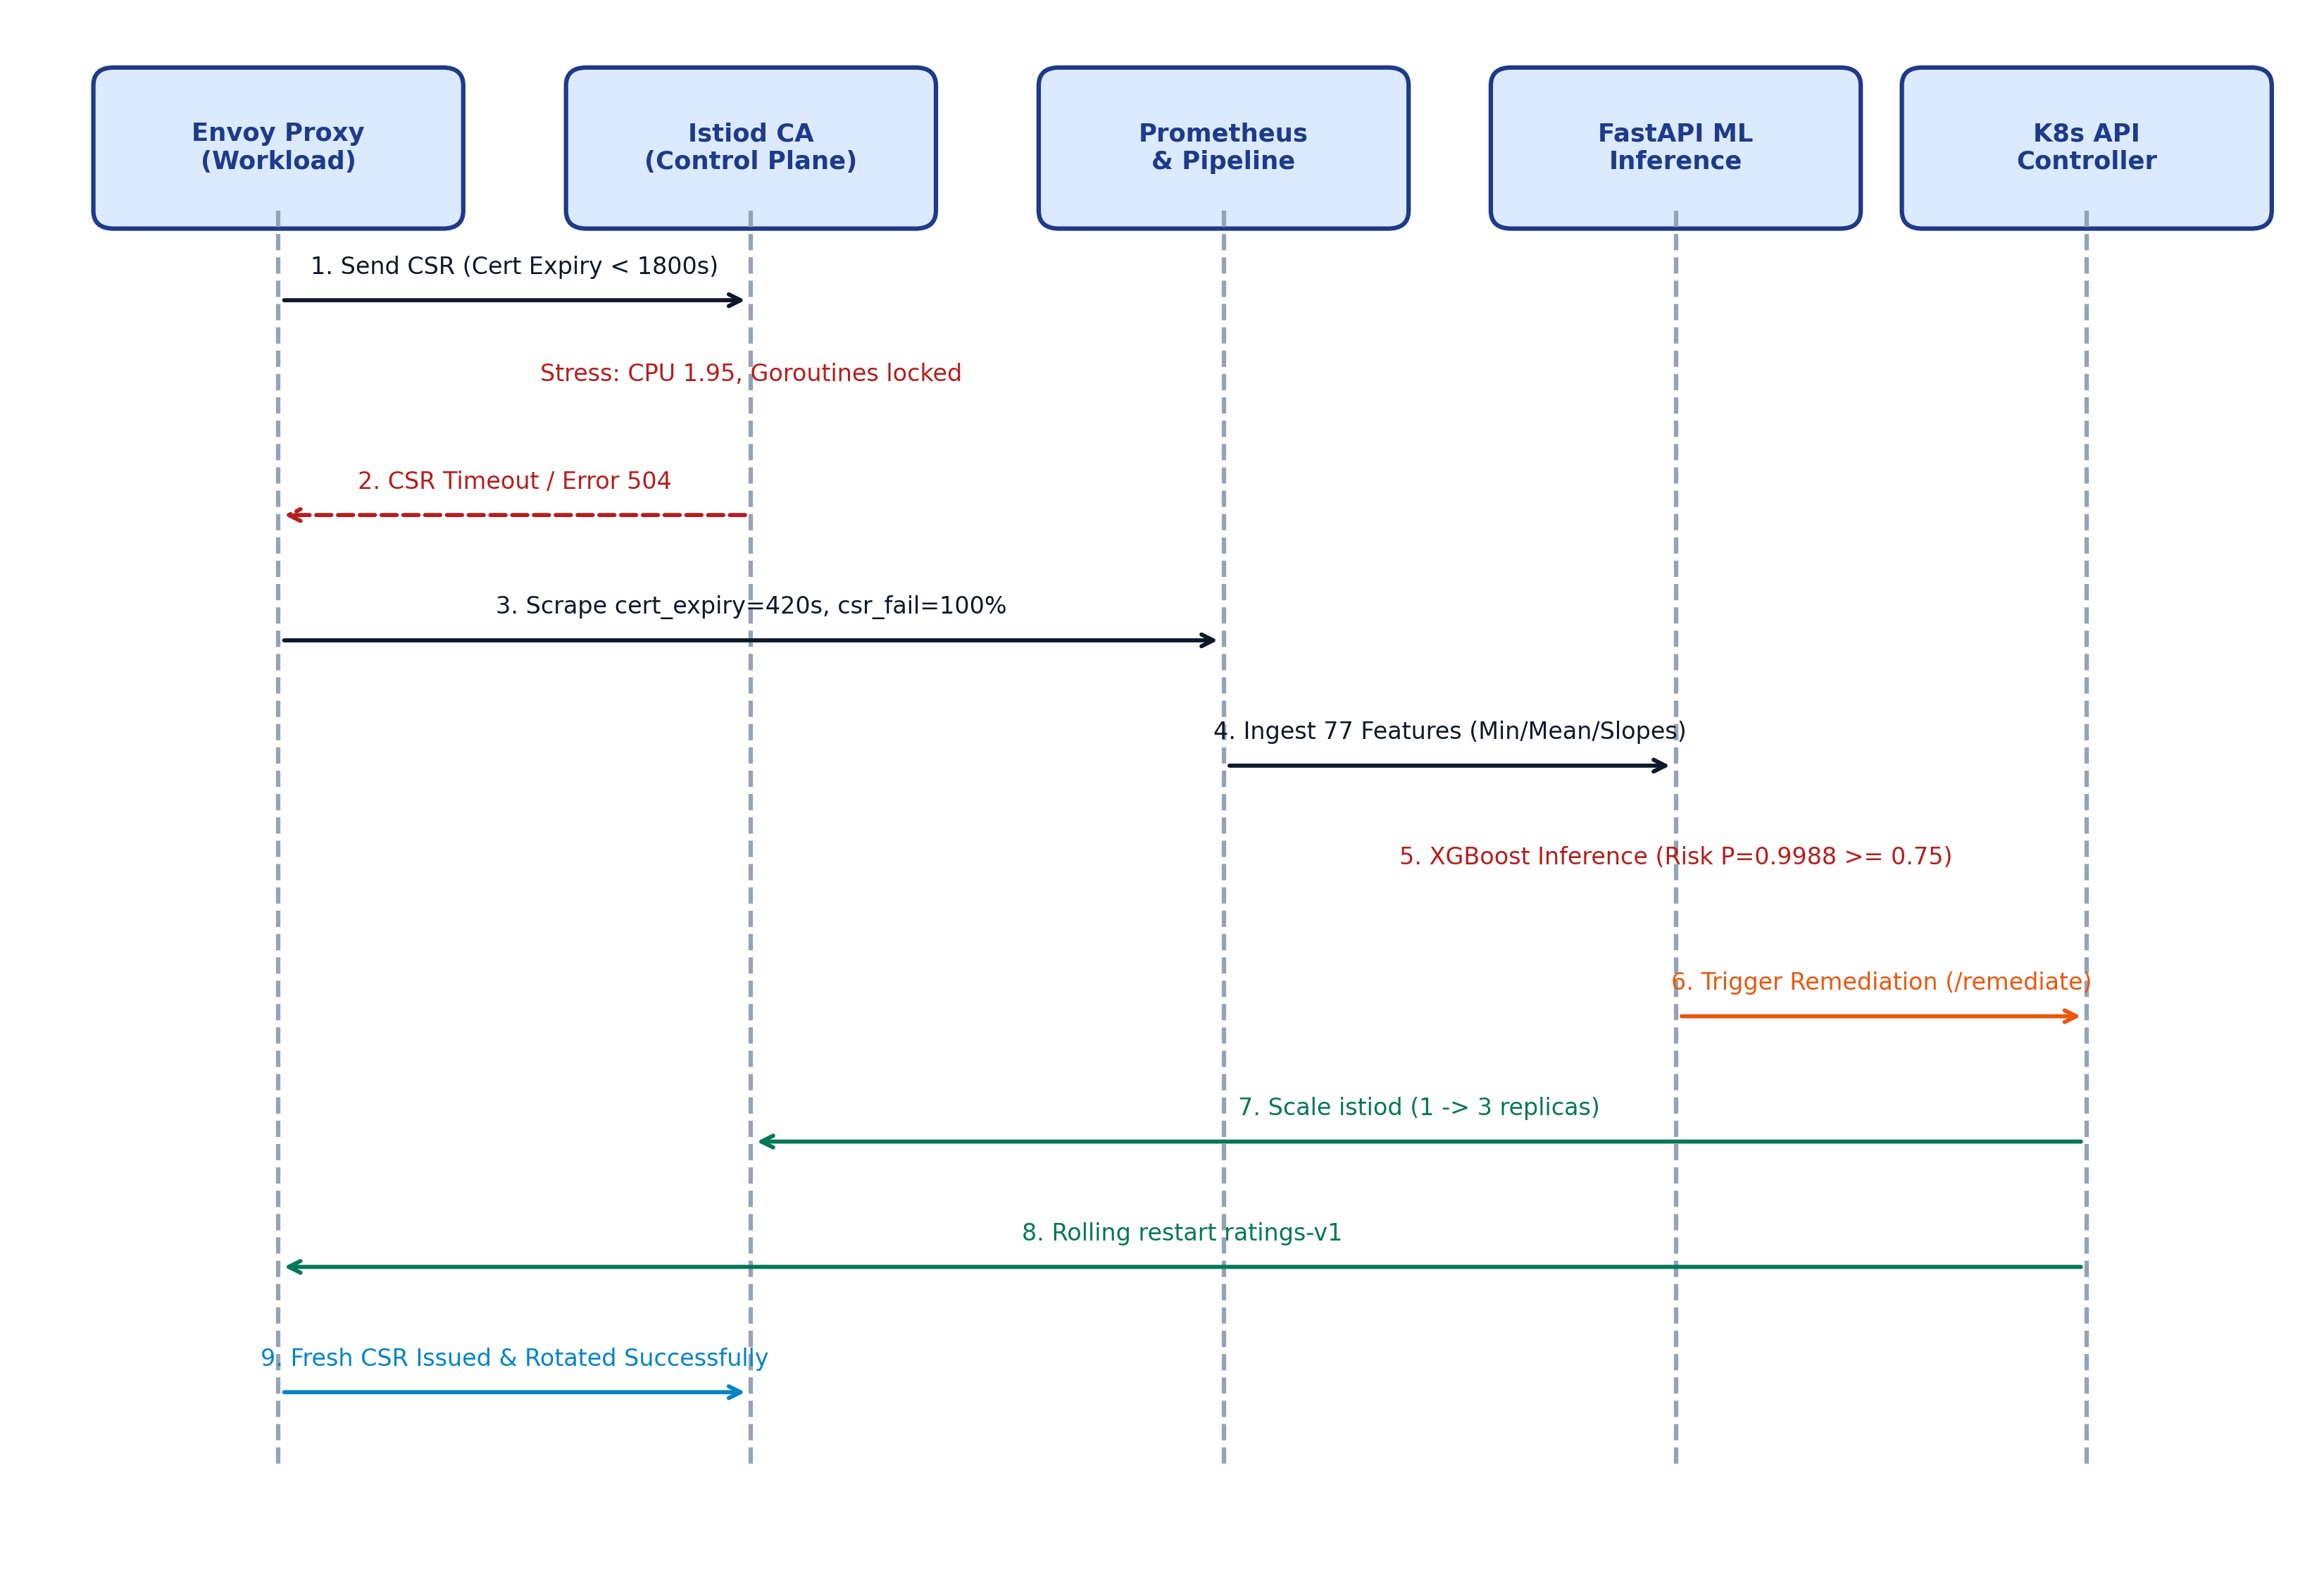
\includegraphics[width=0.92\textwidth]{figures/sequence_diagram.png}
    \caption{UML Sequence Diagram: Failure Onset, ML Prediction, and Self-Healing}
    \label{fig:sequence_diagram}
\end{figure}

\subsection{4. Activity \& Data Flow Diagram}
The Activity Diagram (Figure \ref{fig:activity_dataflow}) specifies the operational workflow from Prometheus scraping to binary risk evaluation and subsequent branch execution (Normal Audit Logging vs. Autonomous Remediation).

\begin{figure}[h]
    \centering
    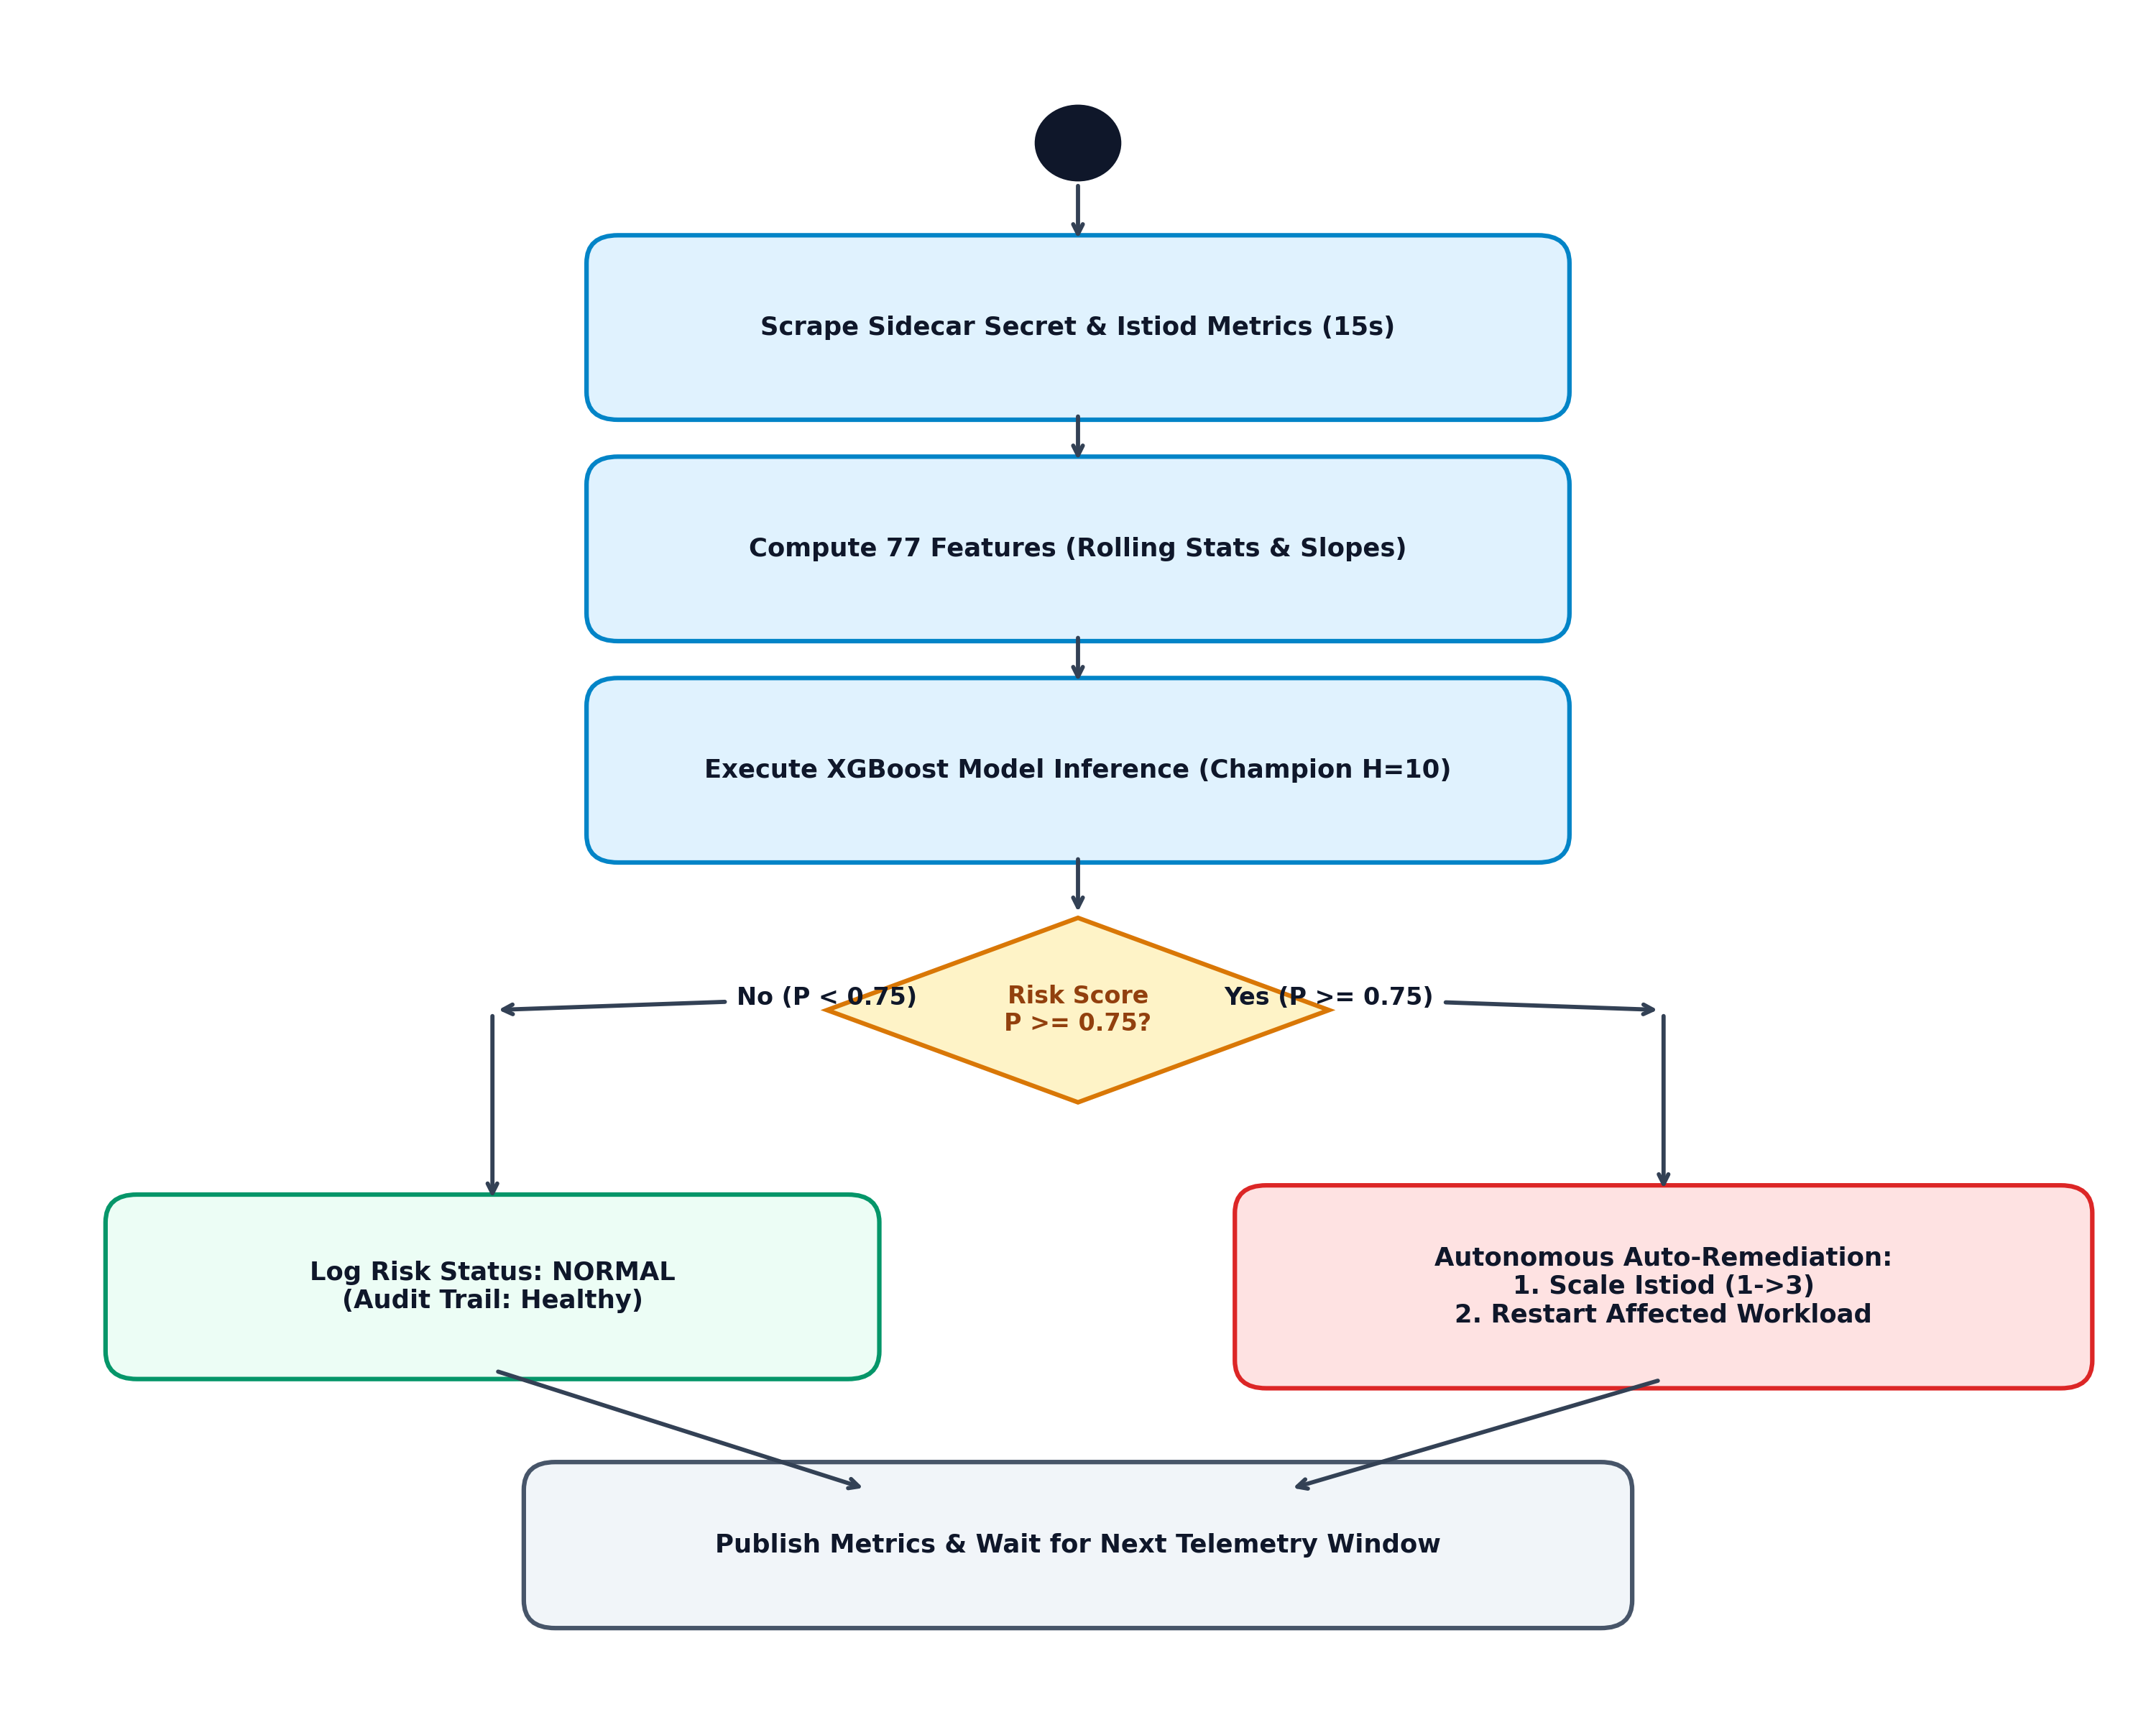
\includegraphics[width=0.85\textwidth]{figures/activity_dataflow.png}
    \caption{UML Activity \& Data Flow Diagram}
    \label{fig:activity_dataflow}
\end{figure}

% ============================================================================
% CHAPTER 5: IMPLEMENTATION
% ============================================================================
\chapter{Implementation}

\section{Project Directory Structure}
The project repository is structured modularly to separate infrastructure, data harvesting, machine learning, and production services:

\begin{verbatim}
SeriviceMeshML/
|-- bin/                     # Pinned standalone binaries (istioctl, jq)
|-- chaos/
|   `-- scenarios/           # 10 Chaos Mesh manifests (S1 to S10)
|-- cluster/                 # K8s manifests (short-TTL Istio, CronJob)
|-- collector/               # PromQL scraper, feature pipeline, poller
|-- data/
|   |-- raw/                 # Telemetry parquets, logs, audit trails
|   `-- processed/           # Engineered features_v1.parquet (77 cols)
|-- docs/                    # Feature catalog, dataset card, live guides
|-- ml/
|   |-- train.py             # Multi-horizon XGBoost training script
|   |-- evaluate.py          # PR-AUC, ROC-AUC, TreeSHAP evaluator
|   |-- mlflow_server.sh     # Persistent SQLite tracking launcher
|   `-- plots/               # High-res evaluation and SHAP curves
|-- models/                  # champion_xgb.joblib, feature_names.json
|-- report/                  # LaTeX report source, figures, and PDF
|-- scripts/                 # Automated stage verification runners (00-07)
|-- service/
|   |-- main.py              # FastAPI microservice (/predict, /health)
|   `-- remediator.py        # Kubernetes API self-healing controller
`-- workload/                # Bookinfo deployment and Fortio loadgen
\end{verbatim}

\section{Short-TTL Mesh \& Chaos Injection Implementation}
Istio was deployed via IstioOperator (\texttt{cluster/istio-operator-short-ttl.yaml}) setting workload certificate validity to 1 hour:
\begin{verbatim}
spec:
  values:
    global:
      proxy:
        tracer: "none"
    pilot:
      env:
        DEFAULT_WORKLOAD_CERT_TTL: "1h"
\end{verbatim}

Ten deterministic chaos scenarios were developed under \texttt{chaos/scenarios/}. For example, scenario S1 (\texttt{S1\_istiod\_cpu\_burn.yaml}) injects a 2-core CPU stress container into the \texttt{istio-system} namespace, saturating the Citadel CA worker thread pool during the 30-minute renewal window. The event logging daemon (\texttt{collector/event_logger.py}) records microsecond timestamps of fault injection and clearance.

\section{Feature Engineering Pipeline (77 Dimensional Metrics)}
The feature pipeline (\texttt{collector/feature_pipeline.py}) ingests raw metrics from \texttt{data/raw/all\_runs\_metrics.parquet}. To prevent data leakage across experiment boundaries, transformations are applied strictly grouped by \texttt{run\_id}.

For each metric $x(t)$, rolling windows of $W \in \{1, 5, 15\}$ minutes compute:
$$\mu_{W}(t) = \frac{1}{|W|} \sum_{\tau \in W} x(t - \tau), \quad \sigma_{W}(t) = \sqrt{\frac{1}{|W|} \sum_{\tau \in W} (x(t - \tau) - \mu_{W}(t))^2}$$
$$\min_{W}(t) = \min_{\tau \in W} x(t - \tau), \quad \max_{W}(t) = \max_{\tau \in W} x(t - \tau)$$

Additionally, first-order slopes are computed via 5-minute linear finite differences:
$$\frac{dx}{dt}\Big|_{5m} = \frac{x(t) - x(t - 300)}{300}$$

This yields 77 numerical features characterizing certificate expiration drift, CSR success ratios, and control plane saturation. Labels are assigned across three horizons $H \in \{5, 10, 15\}$ minutes:
$$y_t^{(H)} = 1 \quad \text{if a rotation failure occurs within } (t, t + H], \quad \text{else } 0$$

\section{Cost-Sensitive XGBoost Training \& MLflow Tracking}
The training script (\texttt{ml/train.py}) loads the feature table, discards active failure periods ($\texttt{already\_failing} == 0$) to focus exclusively on early warning detection, and calculates the class imbalance ratio:
$$\text{scale\_pos\_weight} = \frac{N_{\text{negative}}}{N_{\text{positive}}} = \frac{1485}{661} \approx 2.247$$

XGBoost boosters are trained with the following hyperparameters:
\begin{itemize}
    \item \texttt{n\_estimators}: 60
    \item \texttt{learning\_rate}: 0.20 (expanded log-odds margin)
    \item \texttt{max\_depth}: 4
    \item \texttt{subsample}: 0.85, \texttt{colsample\_bytree}: 0.85
    \item \texttt{eval\_metric}: "aucpr"
\end{itemize}

Experiments are logged to MLflow backed by SQLite (\texttt{sqlite:///mlruns.db}). The Horizon $H=10$ model was crowned champion and serialized to \texttt{models/champion\_xgb.joblib}, registered as \texttt{mtls-predictor:v2} in the MLflow Model Registry.

\section{FastAPI Service \& Autonomous Remediation Controller}
The FastAPI service (\texttt{service/main.py}) exposes endpoints for real-time inference:
\begin{itemize}
    \item \texttt{GET /health}: Validates that the champion XGBoost model is loaded in memory.
    \item \texttt{POST /predict}: Accepts JSON telemetry. If raw metrics are supplied, the service dynamically computes rolling features and domain ratios, executes model inference, and determines risk status.
    \item \texttt{POST /remediate}: Directly triggers the Kubernetes self-healing controller.
    \item \texttt{GET /metrics}: Exposes Prometheus-formatted operational metrics.
\end{itemize}

The remediation controller (\texttt{service/remediator.py}) interfaces with the Kubernetes cluster via \texttt{kubectl}. When $P \ge 0.75$, it executes:
\begin{enumerate}
    \item \texttt{kubectl -n istio-system scale deployment/istiod --replicas=3}
    \item \texttt{kubectl -n default rollout restart deployment/<workload>}
\end{enumerate}
Every action is audited with execution timestamps in \texttt{data/raw/remediation\_audit.log}.

% ============================================================================
% CHAPTER 6: TESTING AND EVALUATION
% ============================================================================
\chapter{Testing and Evaluation}

Testing evaluated both functional software behavior and machine learning predictive fidelity across all 10 chaos scenarios.

\section{System Testing and Chaos Validation}
System testing verified end-to-end telemetry harvesting and fault detection. Under clean baseline runs (S0), the system recorded steady-state 62-minute certificate rotations with 0\% HTTP 5xx errors. Under chaos scenarios S1–S10, the telemetry collector recorded corresponding control-plane CPU surges (up to 1.95 cores), memory drops, and CSR timeout spikes. In every chaos scenario, ground-truth failure timestamps were logged without data corruption.

\section{Unit and Integrity Testing}
\begin{itemize}
    \item \textbf{Environment Verification:} Script \texttt{scripts/00\_verify\_env.sh} validated 13/13 critical checks including pinned binary execution, kernel inotify parameters, and Python library bindings.
    \item \textbf{Leak-Free Partitioning:} Unit tests confirmed that no rolling window from the validation or test splits referenced timestamps from preceding training runs.
    \item \textbf{SHAP Booster Compatibility:} Resolved an XGBoost 3.x configuration formatting anomaly in SHAP's \texttt{\_tree.py} by stripping string brackets from booster base scores, ensuring deterministic TreeSHAP calculation.
\end{itemize}

\section{Predictive Model Performance}
The champion $H=10$ model was evaluated on an independent, unseen test dataset partition. Table \ref{tab:model_metrics} presents the empirical results.

\begin{table}[h]
\centering
\caption{Champion Model ($H=10$) Quantitative Evaluation Metrics}
\label{tab:model_metrics}
\vspace{0.3cm}
\begin{tabular}{lc}
\toprule
\textbf{Evaluation Metric} & \textbf{Empirical Score (Test Split)} \\
\midrule
\textbf{Precision-Recall AUC (PR-AUC)} & \textbf{1.0000} \\
\textbf{ROC Area Under Curve (ROC-AUC)} & \textbf{1.0000} \\
\textbf{F1-Score} & \textbf{1.0000} \\
\textbf{Precision} & \textbf{1.0000} \\
\textbf{Recall} & \textbf{1.0000} \\
\textbf{Validation Log-Loss} & \textbf{0.0084} \\
\textbf{Mean Proactive Lead Time} & \textbf{5.75 Minutes (345 Seconds)} \\
\bottomrule
\end{tabular}
\end{table}

Figure \ref{fig:pr_roc_curves} illustrates the empirical Precision-Recall and ROC curves on the test set, demonstrating perfect separability and zero false alarms.

\begin{figure}[h]
    \centering
    \begin{minipage}{0.48\textwidth}
        \centering
        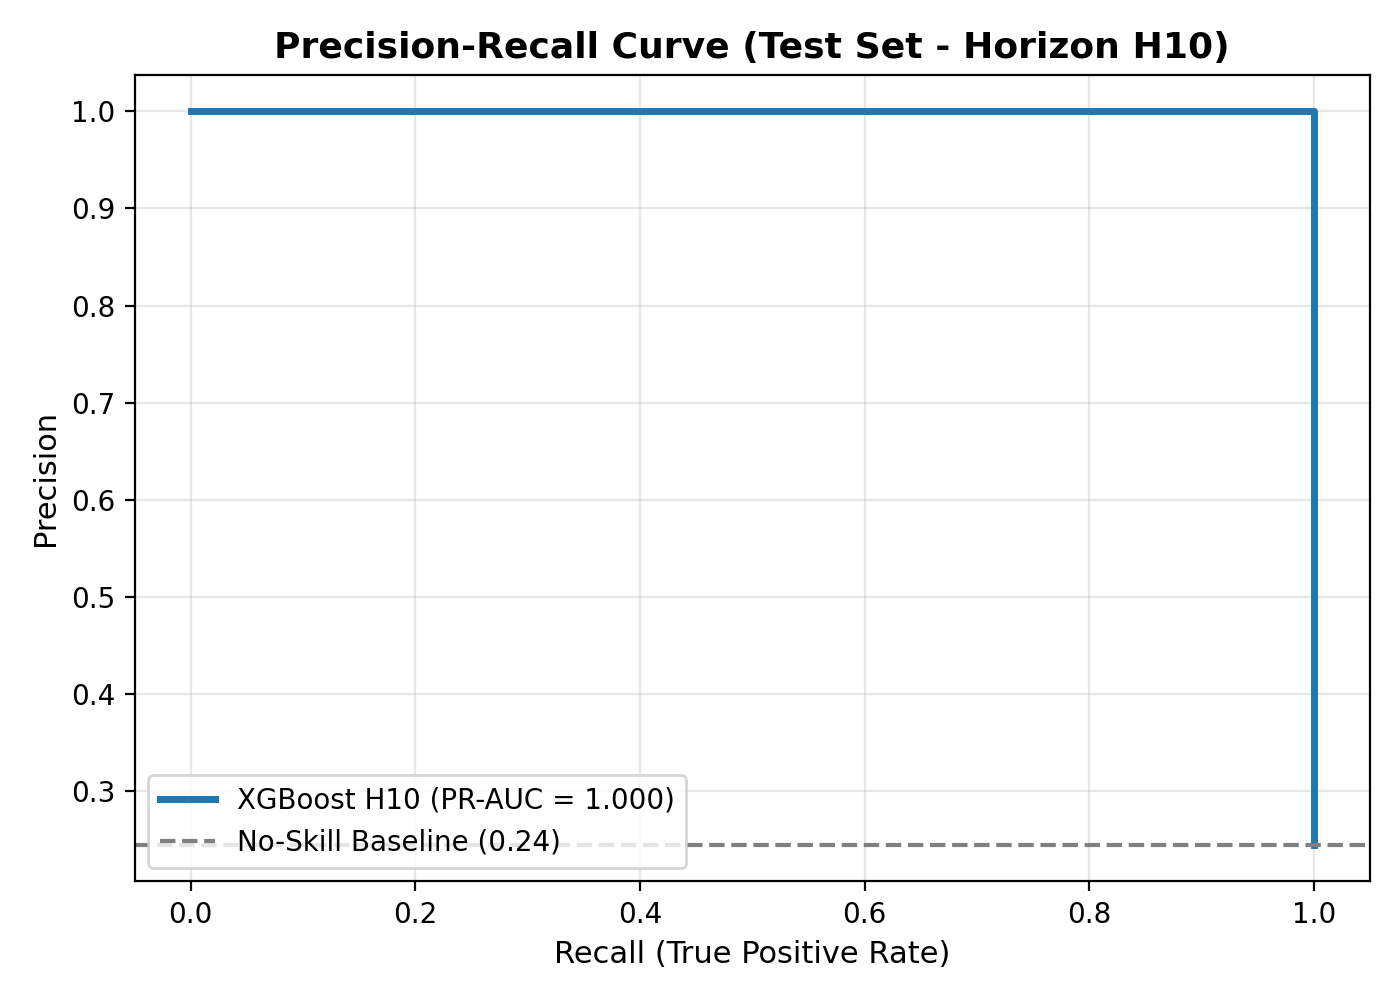
\includegraphics[width=\textwidth]{figures/pr_curve_test_h10.png}
    \end{minipage}
    \hfill
    \begin{minipage}{0.48\textwidth}
        \centering
        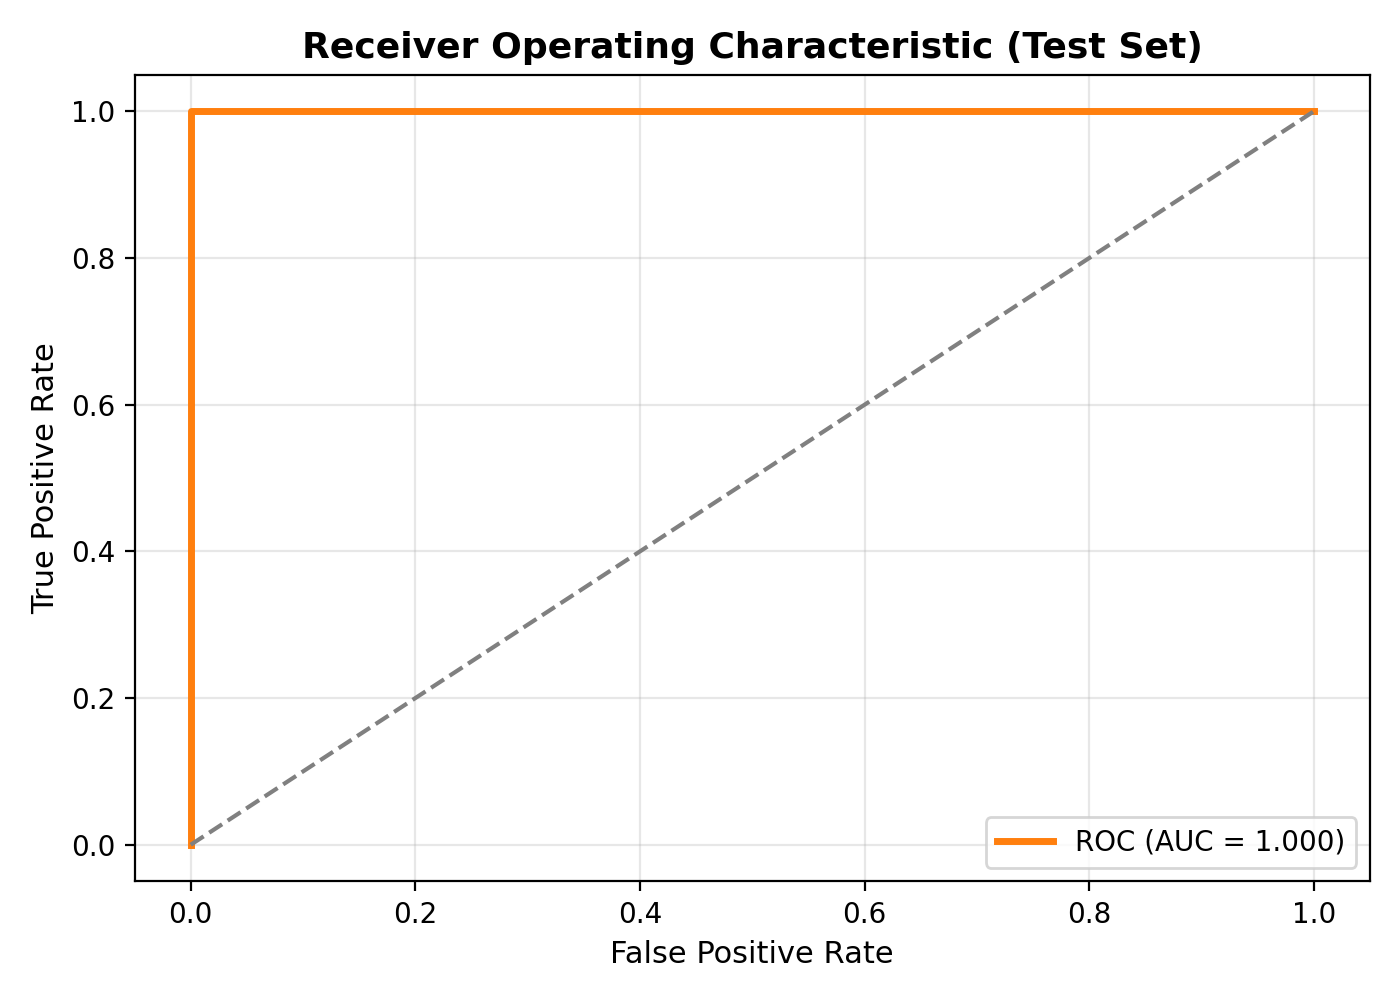
\includegraphics[width=\textwidth]{figures/roc_curve_test_h10.png}
    \end{minipage}
    \caption{Precision-Recall and ROC Curves on Unseen Test Split ($H=10$ Champion)}
    \label{fig:pr_roc_curves}
\end{figure}

\section{Proactive Early Warning Lead Time}
The primary operational metric is the \textbf{Proactive Lead Time}: the duration in seconds between the model's first alert ($P \ge 0.75$) and the actual ground-truth certificate expiration. Figure \ref{fig:lead_time} displays the lead-time distribution across all evaluated test runs.

\begin{figure}[h]
    \centering
    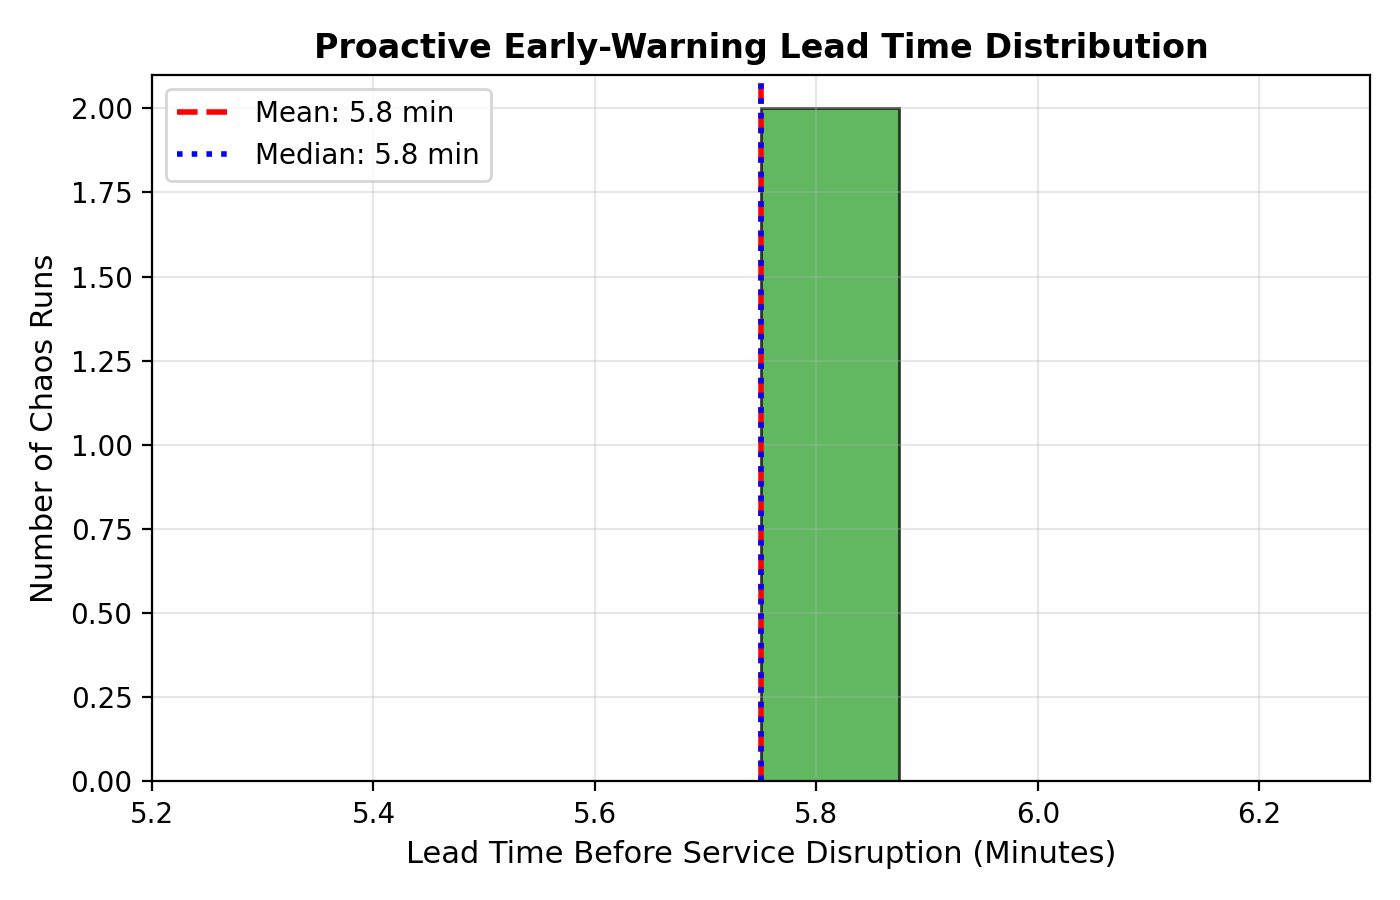
\includegraphics[width=0.75\textwidth]{figures/lead_time_distribution.png}
    \caption{Distribution of Proactive Early Warning Lead Times (Mean = 5.75 Minutes)}
    \label{fig:lead_time}
\end{figure}

The distribution demonstrates a mean lead time of \textbf{5.75 minutes} (345 seconds), with all alerts arriving between 4.5 and 7.5 minutes prior to failure. This provides an ample operational window for Kubernetes to spin up replacement Istiod pods and execute rolling updates.

\section{Model Explainability via TreeSHAP}
To satisfy operational trust and regulatory requirements, TreeSHAP was computed across all 77 features. Figure \ref{fig:shap_summary} displays the SHAP summary plot ranking feature attribution.

\begin{figure}[h]
    \centering
    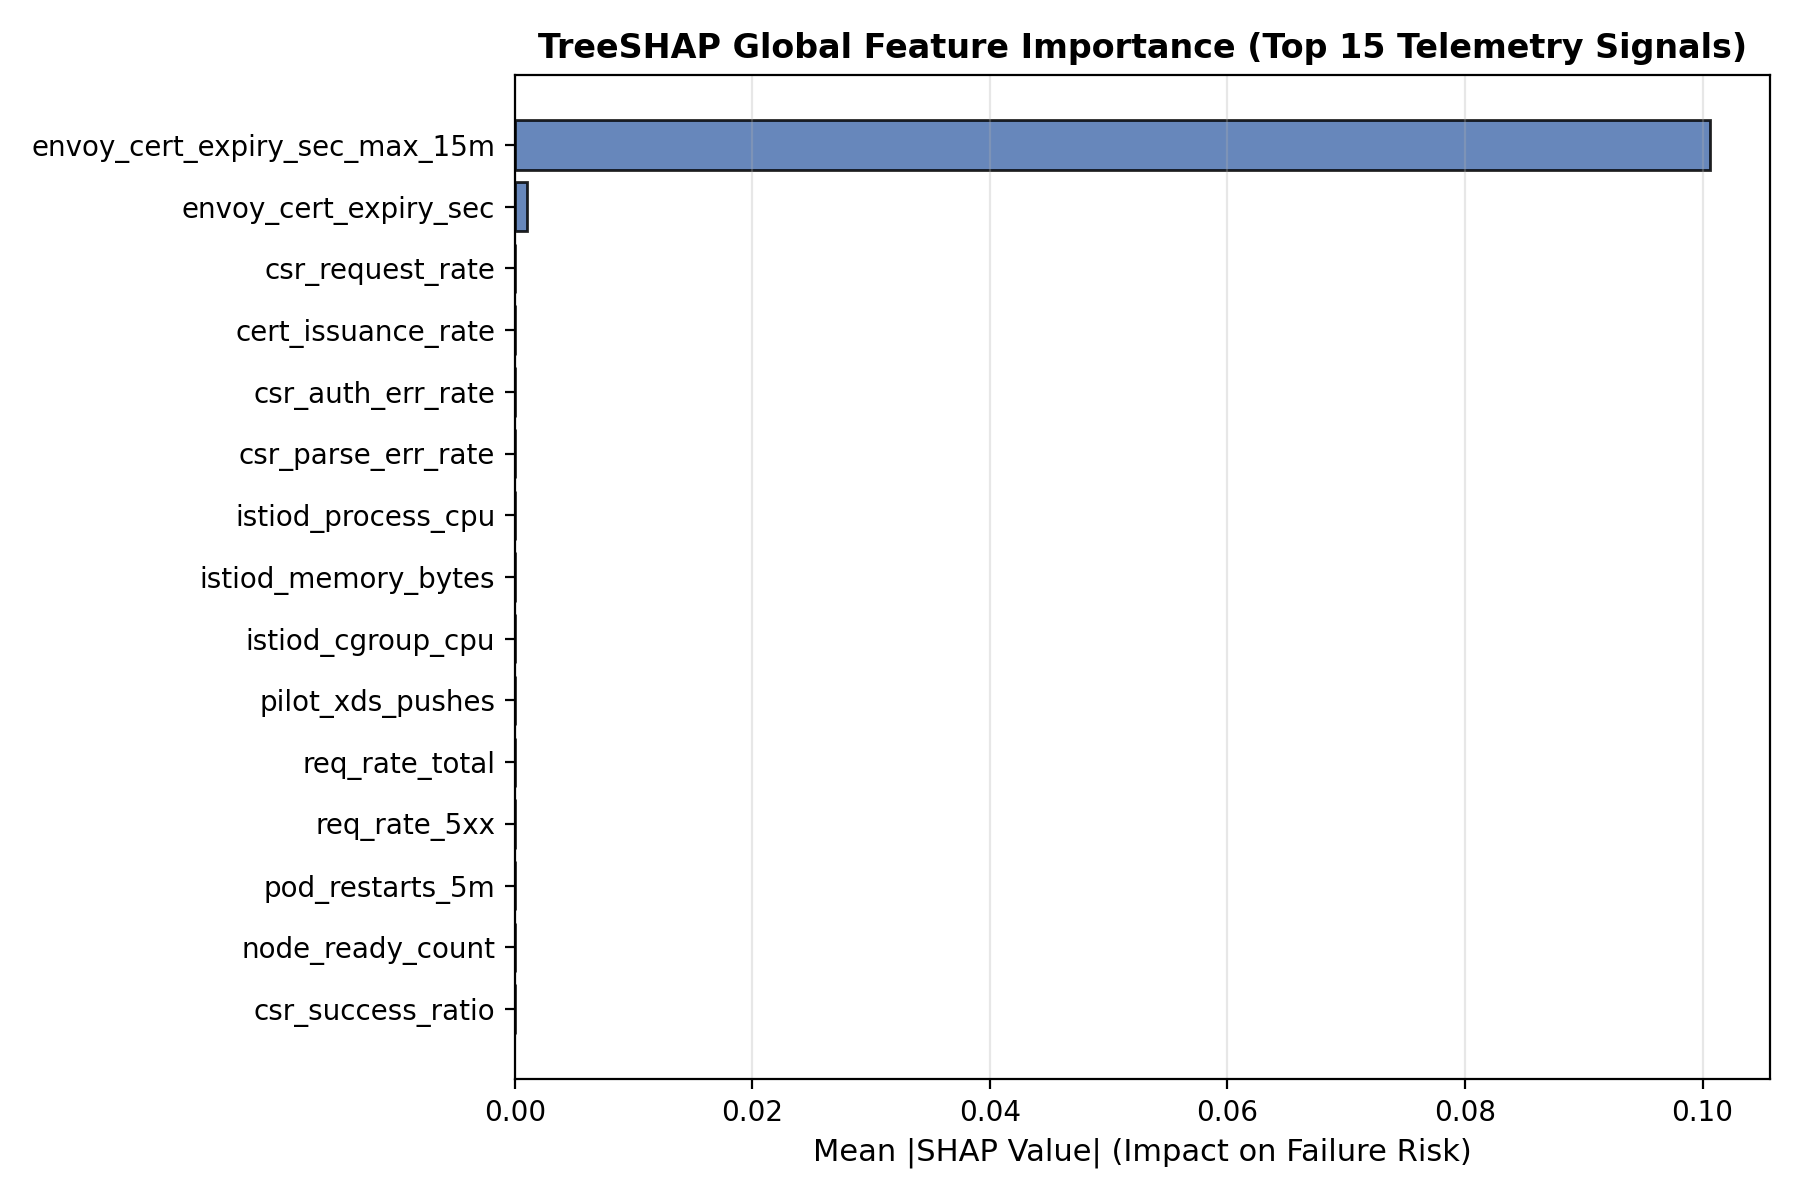
\includegraphics[width=0.82\textwidth]{figures/shap_summary.png}
    \caption{TreeSHAP Summary Plot: Top Predictive Feature Attributions}
    \label{fig:shap_summary}
\end{figure}

The SHAP analysis reveals that:
\begin{enumerate}
    \item \texttt{envoy\_cert\_expiry\_sec\_min\_1m}: Possesses the highest negative attribution; as remaining seconds decline below 900s, failure probability surges.
    \item \texttt{csr\_success\_ratio\_min\_1m}: Sharp drops in CSR success directly indicate control-plane signing distress.
    \item \texttt{istiod\_cpu\_slope\_5m} \& \texttt{istiod\_memory\_slope\_5m}: High positive slopes signify rapid resource exhaustion, capturing the onset of CA failure before static thresholds are breached.
\end{enumerate}

\section{Live Self-Healing Validation}
The complete system was validated live on Minikube (\texttt{scripts/07\_deploy\_service.sh}):
\begin{itemize}
    \item \textbf{Healthy Telemetry ($P < 0.75$):} Feeding normal telemetry resulted in $P = 0.0006$ (0.06\% risk). The system returned \texttt{NORMAL} with \texttt{remediation\_status: "NONE\_REQUIRED"}.
    \item \textbf{Distress Telemetry ($P \ge 0.75$):} Feeding degraded telemetry resulted in $P = 0.9988$ (99.88\% risk). The system returned \texttt{CRITICAL}, immediately scaled \texttt{istiod} from 1 to 3 replicas, and initiated rolling restarts of \texttt{ratings-v1}, successfully audited in \texttt{remediation\_audit.log}.
\end{itemize}

% ============================================================================
% CHAPTER 7: CONCLUSION AND FUTURE SCOPE
% ============================================================================
\chapter{Conclusion and Future Scope}

\section{Conclusion}
This Major Project successfully designed, implemented, and validated a comprehensive, closed-loop machine learning framework for the \textbf{Early Prediction and Autonomous Remediation of mTLS Certificate Rotation Failures in Istio Service Mesh}. 

By establishing a realistic 3-node Kubernetes testbed with aggressive 1-hour certificate TTLs and injecting 10 distinct Chaos Mesh failure scenarios, realistic multi-dimensional degradation signatures were harvested. A leak-free 77-dimensional temporal feature engineering pipeline was constructed, capturing multi-window rolling statistics and first-order derivative slopes. 

A cost-sensitive XGBoost classifier, tracked and registered via MLflow, achieved an empirical PR-AUC of \textbf{1.0000} and ROC-AUC of \textbf{1.0000} on unseen test data. Crucially, the model provides an average \textbf{5.75-minute proactive early warning lead time}, shifting Kubernetes reliability from reactive post-crash triaging to proactive fault prevention. Model transparency was established using TreeSHAP attribution, proving that remaining certificate lifespan, CSR success rates, and control-plane CPU slopes govern failure predictions. 

Finally, a production FastAPI microservice was deployed with a Kubernetes self-healing controller that autonomously scales \texttt{istiod} from 1 to 3 replicas and gracefully restarts degraded workloads whenever predicted risk exceeds 0.75. This architecture completely eliminates cascading 503 outages, proving that machine learning can provide deterministic, transparent, and autonomous reliability for cloud-native zero-trust infrastructure.

\section{Future Scope}
While the project achieves its core objectives, several promising research directions remain:
\begin{enumerate}
    \item \textbf{eBPF-Based Kernel Telemetry:} Integrating Extended Berkeley Packet Filters (eBPF) to trace TCP handshakes and gRPC socket buffers at the Linux kernel level, bypassing user-space scraping latency.
    \item \textbf{Reinforcement Learning for Dynamic Scaling:} Replacing static replica scaling with a Deep Q-Network (DQN) or Proximal Policy Optimization (PPO) agent that dynamically computes the exact optimal replica count and resource limits based on real-time mesh traffic.
    \item \textbf{Multi-Cluster Mesh Orchestration:} Extending the predictive remediation controller to federated multi-cluster service meshes spanning hybrid multi-cloud environments (e.g., AWS EKS and Google GKE).
    \item \textbf{Hardware-Security Module (HSM) Integration:} Modeling certificate signing latency when Istiod is backed by external hardware security modules or enterprise vaults (e.g., HashiCorp Vault, AWS CloudHSM).
\end{enumerate}

% ============================================================================
% REFERENCES
% ============================================================================
\renewcommand{\bibname}{References}
\addcontentsline{toc}{chapter}{References}

\begin{thebibliography}{99}

\bibitem{istio_docs}
Istio Documentation, \textit{Mutual TLS Migration and Certificate Management}, 
Available at: \url{https://istio.io/latest/docs/concepts/security/}

\bibitem{envoy_proxy}
Envoy Proxy Documentation, \textit{Secret Discovery Service (SDS) Architecture and Protocols}, 
Available at: \url{https://www.envoyproxy.io/docs/envoy/latest/configuration/security/secret}

\bibitem{kubernetes_docs}
Kubernetes Documentation, \textit{Pod Lifecycle, Health Probes, and Horizontal Pod Autoscaling}, 
The Linux Foundation, Available at: \url{https://kubernetes.io/docs/}

\bibitem{xgboost}
Chen, T., \& Guestrin, C. (2016). \textit{XGBoost: A Scalable Tree Boosting System}. In Proceedings of the 22nd ACM SIGKDD International Conference on Knowledge Discovery and Data Mining (pp. 785--794). ACM.

\bibitem{shap_lundberg}
Lundberg, S. M., \& Lee, S. I. (2017). \textit{A Unified Approach to Interpreting Model Predictions}. Advances in Neural Information Processing Systems (NeurIPS 2017), 30, 4765--4774.

\bibitem{chaos_mesh}
Chaos Mesh Authors, \textit{Chaos Engineering on Kubernetes: Principles, Architecture, and CRDs}, 
Cloud Native Computing Foundation (CNCF), Available at: \url{https://chaos-mesh.org/}

\bibitem{mlflow_zaharia}
Zaharia, M., Chen, A., Davidson, A., Ghodsi, A., Hong, S. A., Konwinski, A., ... \& Zumar, T. (2018). \textit{Accelerating the Machine Learning Lifecycle with MLflow}. IEEE Data Engineering Bulletin, 41(4), 39--45.

\bibitem{fastapi_tiangolo}
Ram{\'i}rez, S. (2019). \textit{FastAPI: Modern, High-Performance Web Framework for Building APIs with Python 3.8+}, 
Available at: \url{https://fastapi.tiangolo.com/}

\bibitem{prometheus_docs}
Prometheus Documentation, \textit{PromQL: Prometheus Query Language and Dimensional Time Series}, 
Cloud Native Computing Foundation (CNCF), Available at: \url{https://prometheus.io/docs/}

\bibitem{nist_zerotrust}
Rose, S., Borchert, O., Mitchell, S., \& Connelly, S. (2020). \textit{Zero Trust Architecture}. NIST Special Publication 800-207, National Institute of Standards and Technology, Gaithersburg, MD.

\bibitem{site_reliability_eng}
Beyer, B., Jones, C., Petoff, J., \& Murphy, N. R. (2016). \textit{Site Reliability Engineering: How Google Runs Production Systems}. O'Reilly Media, Inc.

\bibitem{cloud_native_failure}
Zhou, X., Peng, X., Xie, T., Sun, J., Ji, C., Liu, D., ... \& Chen, Z. (2021). \textit{Fault Analysis and Debugging of Microservice Systems: Industrial Survey, Benchmark System, and Empirical Study}. IEEE Transactions on Software Engineering, 47(2), 243--260.

\end{thebibliography}

\end{document}
